\documentclass[acmsmall, screen]{acmart}
\setlength{\pdfpagewidth}{8.5in}
\setlength{\pdfpageheight}{11in}
%\settopmatter{printfolios=true,printccs=true,printacmref=true}
\setcopyright{rightsretained}
\acmPrice{}
\acmDOI{10.1145/3360579}
\acmYear{2020}
\copyrightyear{2020}
\acmJournal{PACMPL}
\acmVolume{3}
\acmNumber{OOPSLA}
\acmArticle{153}
\acmMonth{10}

\bibliographystyle{ACM-Reference-Format}
\citestyle{acmauthoryear}   %% For author/year citations
\usepackage{my_style}
\usepackage{listings, wrapfig,xspace}
\usepackage{paralist}
\usepackage{booktabs} % To thicken table lines
\usepackage{makecell}
\usepackage{microtype}

\lstset{language=R}
\definecolor{LightGray}{rgb}{.92,.92,.92}
\definecolor{Gray}{rgb}{.3,.3,.3}
\definecolor{DarkGray}{rgb}{.5,.5,.5}
\lstset{ %
  columns=flexible,
  captionpos=b,
  frame=single,
  framerule=0pt,
  tabsize=2,
  belowskip=0.5em,
  backgroundcolor=\color{LightGray},
  basicstyle=\small\ttfamily,
  emphstyle=,
  keywordstyle=,
  commentstyle=\color{Gray}\em,
  stringstyle=\color{Gray},
%  numbers=left,
  showstringspaces=false
}
\lstdefinestyle{R}{ %
  language=R,
  morekeywords={assign, delayedAssign},
  deletekeywords={env, equal, c, runif, trace, args, exp, t, all},
  breaklines=true
}
\lstdefinestyle{Rin}{ %
  style=R,
  breaklines=false
}
\renewcommand{\k}[1]{{\tt #1}\xspace}


\newcommand{\eg}{\emph{e.g.},\xspace}
\newcommand{\ie}{\emph{i.e.},\xspace}
\newcommand{\cf}{\emph{cf.}\xspace}

\newcommand{\PIR}{\textsf{PIR}\xspace}
\newcommand\pirI[1]{\mathtt{#1}}
\renewcommand{\c}[1]{{\lstinline[style=Rin]!#1!}\xspace}
\newcommand{\code}[1]{{\lstinline[style=Rin]!#1!}\xspace}
% Macros for type names from the old paper.
\newcommand{\attr}[2]{\ensuremath{#1_{\mathtt{#2}}}\xspace}
\newcommand{\attrclass}[3]{\ensuremath{#1^{\mathtt{#3}}_{\mathtt{#2}}}\xspace}
\renewcommand{\to}{\ensuremath{\rightarrow}\xspace}


\newcommand{\nul}{\texttt{\textbf{null}}\xspace}
\newcommand{\scalar}{\texttt{\textbf{scalar}}\xspace}
\renewcommand{\vector}{\texttt{\textbf{vector}}\xspace}
\newcommand{\class}{\texttt{\textbf{class}}\xspace}
\newcommand{\any}{\texttt{\textbf{any}}\xspace}
\newcommand{\environment}{\texttt{\textbf{env}}\xspace}
\newcommand{\expression}{\texttt{\textbf{expression}}\xspace}
\newcommand{\Language}{\texttt{\textbf{lang}}\xspace} %% Upper case!
\newcommand{\externalptr}{\texttt{\textbf{externalptr}}\xspace}
\renewcommand{\symbol}{\texttt{\textbf{symbol}}\xspace}
\newcommand{\pairlist}{\texttt{\textbf{pairlist}}\xspace}
\newcommand{\weakref}{\texttt{\textbf{weakref}}\xspace}
\renewcommand{\int}{\texttt{\textbf{int}}\xspace}
\newcommand{\chr}{\texttt{\textbf{chr}}\xspace}
\newcommand{\dbl}{\texttt{\textbf{dbl}}\xspace}
\newcommand{\lgl}{\texttt{\textbf{lgl}}\xspace}
\newcommand{\clx}{\texttt{\textbf{clx}}\xspace}
\newcommand{\raw}{\texttt{\textbf{raw}}\xspace}
\newcommand{\NA}{\texttt{{NA}}\xspace}
\newcommand{\VARGS}{\texttt{\textbf{...}}\xspace}
\newcommand{\T}{\ensuremath{T}\xspace}
\renewcommand{\S}{\ensuremath{S}\xspace}
\newcommand{\V}{\ensuremath{V}\xspace}
\newcommand{\A}{\ensuremath{A}\xspace}
\newcommand{\ID}{\ensuremath{ID}\xspace}
\newcommand{\F}{\ensuremath{F}\xspace}
\newcommand{\B}{\ensuremath{B}\xspace}
\newcommand{\FUN}[2]{\ensuremath{\langle #1 \rangle \rightarrow #2}\xspace}
\newcommand{\STRUCT}[1]{\texttt{\textbf{struct}}\ensuremath{\langle #1\rangle}\xspace}
\newcommand{\LIST}[1]{\texttt{\textbf{list}}\ensuremath{\langle #1\rangle}\xspace}
\newcommand{\CLASS}[1]{\texttt{\textbf{class}}\ensuremath{\langle #1\rangle}\xspace}
\newcommand{\VEC}[1]{#1\k{[]}}
\newcommand{\NAVEC}[1]{\k{\string^}\!#1\k{[]}}
\newcommand{\NASCA}[1]{\k{\string^}\!#1\xspace}


\newcommand{\contractr}{{\sf ContractR}\xspace} % contractr
\newcommand{\roxygen}{{\sf Roxygen2}\xspace} % roxygen
\newcommand{\typetracer}{{\sf Typetracer}\xspace} % typetracer
\newcommand{\rdt}{{\sf R-dyntrace}\xspace}
\newcommand{\covr}{{\sf Covr}\xspace}



\newcommand {\PercUnitypedPositions} {87.2\%\xspace} %% 0.8717
\newcommand {\PercManytypedPositions} {2\%\xspace} %% 0.018
\newcommand {\CountMonomorphicFunctions} {13.1 K\xspace} %% 13099
\newcommand {\PercMonomorphicFunctions} {64.8\%\xspace} %% 0.648016226377758
\newcommand {\CountPolymorphicFunctions} {7.1 K\xspace} %% 7115
\newcommand {\PercPolymorphicFunctions} {35.2\%\xspace} %% 0.351983773622242

\newcommand{\CranAssertsRnd}{32.3K\xspace}
\newcommand{\CranAsserts}{32,327\xspace}
\newcommand{\CranAssertsInPackagesRnd}{2.4K\xspace}
\newcommand{\CranAssertsInPackages}{2,363\xspace}
\newcommand{\CranAssertsInFunctionsRnd}{15.9K\xspace}
\newcommand{\CranAssertsInFunctions}{15,929\xspace}
\newcommand{\CranStopifnotRatio}{87.6\%\xspace}
\newcommand{\CranTypedAssertsRnd}{12K\xspace}
\newcommand{\CranTypedAsserts}{11,997\xspace}
\newcommand{\CranTypedAssertsRatio}{37.1\%\xspace}
\newcommand{\CranTypedAssertsPackagesRnd}{1.5K\xspace}
\newcommand{\CranTypedAssertsPackages}{1,487\xspace}
\newcommand{\CranTypedAssertsPackagesRatio}{62.9\%\xspace}
\newcommand{\CranTypedAssertsFunctionsRnd}{7.1K\xspace}
\newcommand{\CranTypedAssertsFunctions}{7,119\xspace}
\newcommand{\CranTypedAssertsFunctionsRation}{44.7\%\xspace}
\newcommand{\CranPartiallyTypedAssertsRnd}{15.5K\xspace}
\newcommand{\CranPartiallyTypedAsserts}{15,487\xspace}
\newcommand{\CranPartiallyTypedAssertsRatio}{47.9\%\xspace}
\newcommand{\CranPartiallyTypedAssertsPackagesRnd}{1.7K\xspace}
\newcommand{\CranPartiallyTypedAssertsPackages}{1,664\xspace}
\newcommand{\CranPartiallyTypedAssertsPackagesRatio}{70.4\%\xspace}
\newcommand{\CranPartiallyTypedAssertsFunctionsRnd}{9K\xspace}
\newcommand{\CranPartiallyTypedAssertsFunctions}{9,045\xspace}
\newcommand{\CranPartiallyTypedAssertsFunctionsRation}{56.8\%\xspace}
\newcommand{\CorpusAssertsRnd}{2K\xspace}
\newcommand{\CorpusAsserts}{1,995\xspace}
\newcommand{\CorpusAssertsInPackages}{153\xspace}
\newcommand{\CorpusAssertsInFunctionsRnd}{1.3K\xspace}
\newcommand{\CorpusAssertsInFunctions}{1,264\xspace}
\newcommand{\CorpusStopifnotRatio}{94.7\%\xspace}
\newcommand{\CorpusTypedAssertsRnd}{1K\xspace}
\newcommand{\CorpusTypedAsserts}{1,005\xspace}
\newcommand{\CorpusTypedAssertsRatio}{50.4\%\xspace}
\newcommand{\CorpusTypedAssertsPackages}{114\xspace}
\newcommand{\CorpusTypedAssertsPackagesRatio}{74.5\%\xspace}
\newcommand{\CorpusTypedAssertsFunctions}{688\xspace}
\newcommand{\CorpusTypedAssertsFunctionsRation}{54.4\%\xspace}
\newcommand{\CorpusPartiallyTypedAssertsRnd}{1.2K\xspace}
\newcommand{\CorpusPartiallyTypedAsserts}{1,223\xspace}
\newcommand{\CorpusPartiallyTypedAssertsRatio}{61.3\%\xspace}
\newcommand{\CorpusPartiallyTypedAssertsPackages}{125\xspace}
\newcommand{\CorpusPartiallyTypedAssertsPackagesRatio}{81.7\%\xspace}
\newcommand{\CorpusPartiallyTypedAssertsFunctions}{859\xspace}
\newcommand{\CorpusPartiallyTypedAssertsFunctionsRation}{68\%\xspace}
\newcommand{\AssertthatRevdeps}{211\xspace}
\newcommand{\AssertrRevdeps}{2\xspace}

\newcommand{\KaggleDownloadedRnd}{2.9K\xspace}
\newcommand{\KaggleDownloaded}{2,890\xspace}
\newcommand{\KaggleDuplicatedRnd}{1.1K\xspace}
\newcommand{\KaggleDuplicated}{1,079\xspace}
\newcommand{\KaggleDuplicatedRatio}{37.3\%\xspace}
\newcommand{\KaggleRunnableRnd}{1.8K\xspace}
\newcommand{\KaggleRunnable}{1,811\xspace}
\newcommand{\KaggleRunnableCodeRnd}{131.3K\xspace}
\newcommand{\KaggleRunnableCode}{131,278\xspace}
\newcommand{\KaggleSuccess}{792\xspace}
\newcommand{\KaggleSuccessCodeRnd}{33.7K\xspace}
\newcommand{\KaggleSuccessCode}{33,733\xspace}
\newcommand{\KaggleFailRnd}{2.1K\xspace}
\newcommand{\KaggleFail}{1,019\xspace}
\newcommand{\KaggleErrorMissingLibrary}{0\xspace}
\newcommand{\KaggleErrorTimeout}{0\xspace}


\begin{document}
\title{Designing Types for R, Empirically}
\author{Alexi Turcotte}\affiliation{\institution{Northeastern University}}
\author{Aviral Goel}\affiliation{\institution{Northeastern University}}
\author{Filip Krikava}\affiliation{\institution{Czech Technical University in Prague}}
\author{Jan Vitek}\affiliation{\institution{Northeastern / Czech Technical University}}

\newcommand{\NUMFUNCTIONS}{25,215\xspace}  %%% TODO auto-gen
\newcommand{\NUMPACKAGES}{412\xspace}  %%% TODO auto-gen
\newcommand{\PACKAGES}{412\xspace}  %%% TODO auto-gen
\newcommand{\genthat}{genthat\xspace}  %%% TODO auto-gen
\newcommand{\YEARS}{20\xspace} %%TODO fix
\newcommand{\PERCFAILEDASSERTIONS}{2.05\%\xspace}
\newcommand{\PERCFAILEDASSERTIONSWUNDEF}{1.98\%\xspace}
\newcommand{\PERCASSERTIONSUNDEF}{0.07\%\xspace}
\newcommand{\NUMPKGSEVAL}{8,694\xspace} % autogenerate
\newcommand{\NUMASSERTIONS}{98,105,161\xspace} %autogenerate
\newcommand{\PROPFUNSFAILEDCHECK}{12.29\%\xspace}
\newcommand{\PROPFUNSFAILEDCHECKNOSTHREE}{10.30\%\xspace} 
\newcommand{\PROPARGSFAILINGASSERTS}{2.40\%\xspace} % autogen....
\newcommand{\PERCSUCCARG}{97.60\%\xspace}
\newcommand{\PERCSUCCFUNNOSTHREE}{89.70\%\xspace}
\newcommand{\PERCSUCCFUNS}{87.70\%\xspace}
\newcommand{\PERCCALLSBADFUNSINTESTS}{2.73\%\xspace}
\newcommand{\TOTNUMSIGS}{21,730\xspace}
\newcommand{\PROPSTRUCTSDYN}{65.97\%\xspace}
\newcommand{\NUMFILESRUN}{160,379\xspace}
\newcommand{\NUMFILESREVDEPS}{153,806\xspace}
\newcommand{\NUMFILESKAGGLE}{6,573\xspace}
\newcommand{\NUMNULLASSERTERRORS}{6.46\%\xspace}
\newcommand{\NUMFUNSWITHNULLASSERTERROR}{141\xspace}
\newcommand{\PERCDYNAMICVECERRORS}{12.73\%\xspace}
\newcommand{\NUMFUNSWITHVECASSERTERROR}{114\xspace}
\newcommand{\PERCFAILASSCLASS}{81.44\%\xspace}
\newcommand{\PERCFAILEDONECLASS}{51.13\%\xspace}


% Kaggle
 \newcommand{\PERCFAILEDASSERTIONSKAGGLE}{2.14\%\xspace}
\newcommand{\PERCFAILEDASSERTIONSKAGGLENOUNDEF}{0.42\%\xspace}
 \newcommand{\PROPFUNSWITHFAILEDASSERTKAGGLE}{15.98\%\xspace}
 \newcommand{\NUMTOTALASSERTIONSKAGGLE}{19,038,496\xspace}
 \newcommand{\NUMASSERTEDFUNCTIONSKAGGLE}{970\xspace}

\keywords{type declarations, dynamic languages, R}

\begin{CCSXML}
	<ccs2012>
	<concept>
	<concept_id>10011007.10011006.10011008.10011024</concept_id>
	<concept_desc>Software and its engineering~Language features</concept_desc>
	<concept_significance>500</concept_significance>
	</concept>
	<concept>
	<concept_id>10011007.10011006.10011008</concept_id>
	<concept_desc>Software and its engineering~General programming languages</concept_desc>
	<concept_significance>300</concept_significance>
	</concept>
	<concept>
	<concept_id>10011007.10011006.10011008.10011009.10011021</concept_id>
	<concept_desc>Software and its engineering~Multiparadigm languages</concept_desc>
	<concept_significance>100</concept_significance>
	</concept>
	</ccs2012>
\end{CCSXML}

\ccsdesc[500]{Software and its engineering~Language features}
\ccsdesc[300]{Software and its engineering~General programming languages}

\begin{abstract}
The R programming language is widely used in a variety of domains.  It
was designed to favor an interactive style of programming with minimal
syntactic and conceptual overhead. This design is well suited to data
analysis, but a bad fit for tools such as compilers or program
analyzers. In particular, R has no type annotations, and all
operations are dynamically checked at run-time. The starting point for
our work are the twin questions: \emph{what expressive power is needed
to accurately type R code?} and \emph{which type system is the R
community willing to adopt?} Both questions are difficult to answer
without actually experimenting with a type system. The goal of this
paper is to provide data that can feed into that design process. To
this end, we perform a large corpus analysis to gain insights in the
degree of polymorphism exhibited by idiomatic R code and explore
potential benefits that the R community could accrue from a simple
type system.  As a starting point, we infer type signatures for
\NUMFUNCTIONS functions from \NUMPACKAGES packages among the most
widely used open source R libraries. We then conduct an evaluation on
\NUMPKGSEVAL clients of these packages, as well as on end-user code
from the Kaggle competition.
\end{abstract} \maketitle

\section{Introduction}

Our community builds, improves, and reasons about programming
languages. To make design decisions that benefit users, we need to
understand our target language as well as the real-world needs it
answers. Often, we can appeal to intuition, as many languages are
intended for general purpose programming tasks.  Unfortunately,
intuition may fail us when looking at domain-specific languages
designed for a particular group of users to solve specific needs. This
is the case of the data science language R.

R and its ancestor S were designed, implemented, and maintained by
statisticians. Originally they aimed to be glue languages for 
statistical routines written in Fortran. Over three decades they
became widely used across many fields for exploratory data analysis.
Modern R, as an object of study, is fascinating. It is a vectorized,
dynamically typed, lazy functional language with limited side-effects,
extensive reflective facilities and retrofitted object-oriented programming
support.

Many of the design decisions that gave us R were intended to foster an
interactive and exploratory programming style. These include, to name
a few salient ones, the lack of type annotations, the ability to use
syntactic shortcuts, and widespread conversion between data
types. While these choices have decreased the barrier to entry---many
data science educational programs do not teach R itself but simply
introduce some of its key libraries---they also allow for errors to go
undetected.

Retrofitting a type system to the R language would increase our assurance in
the result of data analysis, but this requires facing two challenges. First,
it is unclear what would be the \emph{right} type system for a language as
baroque as R. For example, one of the most popular data type, the
\code{data.frame}, is manipulated through reflective operations---a data
frame is a table whose columns can be added or removed on the fly.  Second,
but just as crucially, designing a type system that will be adopted would
require overcoming some prejudices and educating large numbers of users.

The goal of this paper is to gather data that can be used as input to
the process of designing a type system for R.  To focus our work, we
chose to limit the scope of investigation on the design of a language
for function type signatures.  Thus, this paper will use the collected
data to document the signature of user-defined functions.  For this,
we design a simple type language, one that matches the R data types.
We then extract call and return types from execution traces of a
corpus of widely used libraries, and finally synthesize type
signatures.  This allows us to see how far one can get with a simple
type language and identify limitations of our design. We validate the
robustness of the extracted type signatures by implementing a contract
checker that weaves types around their respective functions, and use
clients of the target packages for validation.  To sum up, we make the
following contributions:
\begin{itemize}
\item We implemented scalable and robust tooling to automatically
  extract type signatures and instrument R functions with checks
  based on their declared types.
\item We carried out a corpus analysis of \PACKAGES widely used and
  maintained packages to synthesize function type signatures and
  validated the robustness of the signatures against \NUMFILESRUN
  programs that use those functions.
\item We report on the appropriateness and usefulness of a simple type
  language for R.
\item Our data and code are open source and publicly
  available.\footnote{ \url{github.com/PRL-PRG/propagatr},
  \url{github.com/PRL-PRG/contractr}, data: \url{doi.org/10.5281/zenodo.4091818}, artifact: \url{doi.org/10.5281/zenodo.4037278}}
\end{itemize}

%
\section{Background} %%%%%%%%%%%%%%%%%%%%%%%%%%%%%%%%%%%%%%%%%%%%%%%%%%%%%%%%%

This section introduces related work and gives a short primer on R.

\subsection{Related Work} %%%%%%%%%%%%%%%%%%%%%%%%%%%%%%%%%%%%%%%%%%%%%%

Dynamic programming languages such as Racket, JavaScript, PHP and Lua
have been extended post factum with static type systems.  In each
case, the type system was carefully engineered to match the salient
characteristics of its host language and to foster a particular
programming style. For example, Typed Racket emphasizes functional
programming and migration from untyped to fully typed
code~\cite{tf-popl08}, Hack~\cite{hack13} and TypeScript~\cite{BAT14}
focus on object-oriented features of PHP and JavaScript,
respectively. They allow users to mix typed and untyped code in a
fine-grained manner.  In the case of Lua~\cite{typedlua2014}, the type
system tried to account for the myriad ways Lua programmers use
tables.  Other languages adopted a mix of typed and untyped code by
design. In Julia, type annotations are needed for method dispatch and
performance~\cite{oopsla18a}. In Thorn, users could freely move
between typed and untyped code thanks to the addition of like
types~\cite{popl10}. Lastly C\# is an example of a statically typed
language which added a dynamic type~\cite{Bierman10}.

But what if the design of the type system is unclear?  \citet{tip} propose
a promising approach called trace typing. With trace typing, a new type
system can be prototyped and evaluated by applying the type rule to
execution traces of programs. While the approach has the limitation of
dynamic analysis techniques, namely that the results are only as good at the
coverage of the source code, it allows one to quickly test new design and
quantify how much of a code base can be type-checked.  Other approaches that
infer types for dynamic analysis include the work of \citet{FurrAF2009} and
\citet{hicks2011ruby} for Ruby.

Recent work has gone into adding types to Python, the other eminent
data science language.  Typilus is an interesting piece of recent work
which explores using neural networks to infer types for Python
programs~\cite{allamanis2020typilus}, and Python itself added support
for type hints in Python 3.5~\cite{pythonspectypes}.  There is no
previous work on types for R. We take inspiration in the
aforementioned works but focus on adapting them to our target
language.


\subsection{The R Language} %%%%%%%%%%%%%%%%%%%%%%%%%%%%%%%%%

The R Project is a key tool for data analysis.  At the heart of R is a
vectorized, dynamic, lazy, functional, object-oriented language with
an unusual combination of features~\cite{ecoop12}.  R was designed by
\citet{R96} as a successor to S~\cite{S88}.

R's main data type is the primitive vector.  Vectors care explicitly
constructed by the constructor \code{c(...)}, as in \code{c(1L, 2L,
  3L)} which creates a vector of three integers.  R has a builtin
notion of type that can be queried by the \k{typeof}
function. Figure~\ref{rtypes} lists all of the builtin types that are
provided by the language; these are the possible return values of
\k{typeof}. There is no intrinsic notion of subtyping in R, but in
many contexts a \k{logical} will be coerced to \k{integer}, and an
\k{integer} will be coerced to \k{double}.  Some odd conversions can
occur in corner cases, such as \k{1<"2"} holds and \k{c(1,2)[1.6]}
returns the first element of the vector, as the double is converted to
an integer. R does not distinguish between scalars and vectors (they
are all vectors), so \code{typeof(5) ==} \code{typeof(c(5)) ==
  typeof(c(5,5))} \code{ == "double"}.  With the exception of lists,
all vectorized data types are monomorphic.  A \k{list} can hold values
of any other type including \k{list}. For all monomorphic data types,
attempting to store a value of a different type will cause a
conversion. Either the value is converted to the type of the vector,
or the vector is converted to the type of the value.

\begin{wrapfigure}{r}{6.1cm}
\footnotesize\begin{tabular}{l@{}l@{}}\hline
\bf Vectors:\\\hline
\k{logical}   & vector of boolean values\\
\k{integer}   & vector of 32 bit integer values\\
\k{double}    & vector of 64 bit floating points\\
\k{complex}   & vector of complex values\\
\k{character} & vector of strings values\\
\k{raw}       & vector of bytes\\
\k{list}      & vector of values of any type\\\hline
{\bf Scalars:}\\\hline
\k{NULL}      &  singleton null value\\
\k{S4}        &  instance of a S4 class \\
\k{closure}   &  function with its environment\\
\k{environment}& mapping from symbol to value \\\hline
{\bf Implementation:}\\\hline
\k{special},
\k{builtin}, &\k{symbol}, \k{pairlist}, \k{promise}\\
\k{language}, \k{char}, \k{...}, & \k{~any}, \k{expression},\\
\k{externalprt},& \k{bytecode}, \k{weakref}\\\hline
\end{tabular}\caption{Builtin Types}\label{rtypes}\end{wrapfigure}

\noindent
All vectorized data types have a distinguished missing value denoted
by \code{NA} (for ``not available'').  The type of \code{NA} is
\k{logical} (\code{typeof(NA)=="logical"}), but \k{NA} inhabits every
type: \code{typeof(c(1,NA)[2])} \k{==} \k{"double"}.  R also has a
\code{NULL} value.  In data science, it is useful to have a notion of
a ``missing observation'', since vectors are monomorphic there is a
need for a missing value to inhabit each primitive type. In a sense,
\code{NA} represents a missing data point, and \code{NULL} is a
missing data set.

Over time, programmers have found the need for a richer type
structure.  R supports this with {\it attributes}. One may think of
attributes as an optional map from names to values attached to any
built in type.  Attributes are used to encode various type
structures. They are queried with \k{attributes} and \k{class}.  Using
attributes, programmers can extend the set of types by tagging
data. For example, take the vector of four values,
\code{x<-c(1,2,3,4)} and attach attribute \k{dim},
\code{attr(x,"dim")<-c(2,2)}, to treat \k{x} as a 2x2 matrix.

Another attribute that can be set is the \k{class}, this is one way to
use R for object-oriented programming.  This attribute can be bound to
a list of class names. For instance, \code{class(x)<-"human"} will set
the class of \k{x} to be \k{human}.  There are three
object-orientation frameworks in R: S3, S4, and R5.  The S3 object
system support single dispatch on the class of the first argument of a
function, whereas the S4 object system allows multiple dispatch. R5
allows for users to define objects in a more imperative style. Some of
the most widely used data types leverage attributes, e.g., data frames
and matrices. A data frame, for instance, is a list of vectors with a
class and a column name attribute, and matrices are vectors with a
 \k{dims} attribute.


R functions have a number of quirks.  Arguments can be assigned
arbitrary expressions as default values; functions take variable
numbers of parameters, and can be called positionally and nominally.
Consider this example:

\begin{lstlisting}
 f <- function(x,..., y=if(z==0) 1, z=0) { x + y + if(missing(...)) 0 else c(...) }
\end{lstlisting}

\noindent
This function has four formal parameters, \k x, dots, \k y and \k
z. Parameter \k x can be bound positionally or passed by name. The
dots, \k{...}, is always positional. The remaining two parameters must
be passed by name as they are preceded by dots; \k y and \k z have
default values, in the case of \k z this is a constant, but \k{y} is
bound to an expression that depends on \k z's value (if \k z is not
zero, \k y defaults to \k{NULL}). The body of the function will add \k
x and \k y tp either 0 or the result of concatenating the dots into a
primitive vector. The function \k{missing} tests if a parameter was
explicitly passed. The following are some valid invocations of \k f:

\begin{lstlisting}
 > f(1)    
   [1] 2             # a double vector, y is 0, ... is missing
 > f(2, 3, x=1)
   [1] 4 5           # a double vector, y is 0, ... is 2, 3
 > f(x=1, y=1)
   [1] 2             # a double vector, y is 1, ... is missing
 > f(x=1, z=1)
   numeric(0)        # a double vector of length 0, y is NULL
 > f(1L, 2L, y=1L)
   [1] 4             # an integer vector, y is integer 1, ... is integer 2
 > f(1, y=c(1,2))
   [1] 1 2           # a double vetor, y is 1, 2, ... is missing
\end{lstlisting}

\noindent
The above hints at polymorphism: \k f may return a vector of integers
or of doubles of length equal to the max length of its arguments.

%%%%%%%%%%%%%%%%%%%%%%%%%%%%%%%%%%%%%%%%%%%%%%%%%%%%%%%%%%%%%%%%%%%%%%%%%%%%%%
\section{A Type Language for R}%%%%%%%%%%%%%%%%%%%%%%%%%%%%%%%%%%%%%

In this section, we set out to propose a candidate design for a type
language to describe the signatures of R functions.  The goal is not
to propose a final design, but rather a starting point for an
iterative process.

Given the pecularities of the language there are a number of design
choices that need to be reviewed and evaluated. It is not
controversial to include types that cover the six kinds of primitive
vectors, furthermore environments and the distinguished null types are
commonly used and must be included.  Environments are lists with
reference semantics: mutating a value in an environment is performed
in-place.  They are used to store variables and to escape from the
copy-on-write semantics of other data types.  For simplicity, we omit
some of the data types that closer to the implementation of the
language. Fig.~\ref{types} presents our type language.

\begin{figure}[!h] \noindent \small  \centering\begin{minipage}{.45\linewidth}
\begin{tabular}{lclr}
\T& ::= & \any          & \it top type\\
  & |   & \nul         & \it null type\\
  & |   & \environment  & \it environment type \\
  & |   & \S            & \it scalar type \\
  & |   & \V            & \it vector type \\
  & |   & \T~\k{|}\T    & \it union type \\
  & |   & \k{?} \T      & \it nullable type \\
  & |   & \FUN{A_1, \dots~ A_n}\T    & \it function type \\
  & |   & \LIST\T                  & \it list type\\
  & |   & \CLASS{ID_1, \dots~ ID_n}  & \it class type\vspace{5pt}\\
\end{tabular}\end{minipage}   \hfill
\begin{minipage}{.45\linewidth}\begin{tabular}{lclr}
\A & ::= & \T          & \it arguments \\
   & |   & \VARGS      & \it dots \vspace{5pt} \\
\V & ::= & ~\VEC\S     & \it vector types\\
   & |   & \NAVEC\S    & \it na vector types \vspace{5pt}\\
\S & ::= & \int        & \it integer\\
   & |   & \chr        & \it character\\
   & |   & \dbl        & \it double \\
   & |   & \lgl        & \it logical\\
   & |   & \clx        & \it complex \\
   & |   & \raw        & {\it raw } \vspace{5pt}\\%
\end{tabular}\end{minipage}\caption{The R type language}\label{types}
\end{figure}

\paragraph{Scalar} While R does not have scalar data types, there are
cases where functions except scalar values, for example a conditional
takes a single logical (and will complain if more values are passed).
We considered tracking dimensions of data structures, but decided
against it. Instead, the type language differentiates between vectors
of lenght 1 and vectors of any dimension.  The primitive types can be
either vectors (e.g., \VEC\int) or scalars (e.g., \int).  A vector can
happen to be of length 1, and thus a scalar is also a vector.  Vectors
are monomorphic, a vector of doubles contains only doubles.

\paragraph{Missing} 
Each of basic types has its specific \NA. Many built-in functions,
especially those implemented in C or Fortran, do not support \NA
values.  It is thus advantageous to distinguish between vector that
can contain missing values and those that are guaranteed not to.  In
our experience, functions that expect scalar values tend to not admit
{\NA}s, thus scalar types are treated as being \NA-free. The type
language does allows to write \VEC\int to specify that a vector of
integers may have {\NA}s and \NAVEC\int to say that a vector must not
have missing values. Of course, a value of type \VEC\int may happen to
not have any \NA and thus be of type \NAVEC\int.  The type \raw does
not allow {\NA}s, so \VEC\raw is \NA-free.

\paragraph{Nullable} 
The \nul type is inhabited by a singleton \code{NULL} value often used
as a sentinel. Unlike in some other lanugage, \k{NULL} is not the
default value of uninitialized variables. R has different notion for
that (which we do not cover here).  To capture common uses, of
\k{NULL}, the type language has a nullable type, written \code{?}\T.
Values of this type can be either values of type \T or \k{NULL}.

\paragraph{Lists} Heterogeneous collections are implemented using lists.
Lists and vectors are closely related: a vector converts to a list
with \code{as.list}, and lists to vectors with \code{unlist}
(coercions may ensue). The type language allows to specify that a
value is a list containing element of some type \T, written \LIST\T. R
does not have built-in type tests for this purpose, to establish the
type of a value requires traversal and checking individual elements.

\paragraph{Class}
R has three objects systems, code-named S3, S4 and R5. All of them
operate by adding a class attribute to values. The most widely used
system, by far, is S3 which supports single dispatch and multiple
classes~\cite{ecoop12}. The challenge from a type system point of view
is that a value such as integer 5, could be attributed with a class.
Code that performs dispatch would use the class attribute while code
that does not would view the value as an integer. The type language
focuses on the attribute and will hide the underlying type of the
value. While that seems to match common usage it does represent a loss
of expressiveness. The type language also focuses on S3, we leave the
other object systems for future work. S3 has no notion of inheritance,
each value has a list of classes. The type language thus allows to
write \CLASS{\ID_1,\dots,\ID_n} to denote values tagged with the class
names $\ID_1$ to $\ID_n$.

\paragraph{Union} We support untagged unions of types written
$\T_1 \k{~|~} ... \k{~|~} \T_n$. The elements of unions are not
disjoint, 1L is both an \int, a \VEC\int and a \NAVEC\int. R does not
provide a built-in type testing mechanism, e.g. for the case of
\NA-free data types, it is necessary to scan vectors to find out if
they have missing values.

\paragraph{Function}
Functions signatures the form \FUN{A_1, \dots, A_n}\T where each
$\A_i$ argument is either a type \T or \VARGS, a variable length
argument list. Moreover, a single function's signature can be the
disjunction of a number of individual signatures.

\subsection{Subtyping}

The choice of type language follows the structure of values.  The
presence of \NA-free data types and scalars are two choices that must
be validated in practice.  Nullable types are just a special case of
unions.

While R does not support the notion of subtyping between values.  The
conversions between primitive types give us a starting point (e.g., an
\int is always accepted where a \dbl is expected). Furthermore, the
types introduced above induce some the rules of Figure~\ref{fig:sub}:
a vector without \NA is a subtype of a vector, a value of type \T is a
subtype of a nullable \T, a list is subtype of another list if their
elements are subtypes, and a scalar is a subtype of a vector of the
same primitive type.

\begin{figure}[h!tb]\begin{tabular}{rclll}
  \NAVEC\S  & <:& \VEC\S \\
  \T        & <:& \k{?}\T \\
  \LIST{\T} & <:& \LIST{\T'} & \it{iff} \T <: \T' \\
  \S        & <:& \VEC\S \\
  \lgl      & <:& \int\\
  \int      & <:& \dbl\\
  \dbl      & <:& \clx\\  
\end{tabular}
\caption{Subtyping}\label{fig:sub}
\end{figure}


\subsection{Synthesizing signatures}

In order to keep the type signatures compact, we will compact union of
arrows into a single top-level arrow with unions at each argument
position. Thus, the shape of function signatures will be as follows:

\vspace*{1mm}
\FUN{ T_{1,1} \k{~|~} T_{1,i}, \dots, T_{n,1} \k{~|~} T_{n,j}}{T_1 \k{~|~} ... \k{~|~} T_k}
\vspace*{1mm}

\noindent
In other words, we take the union of the types occurring at individual
argument positions rather than an union of function
types. Furthermore, we apply some transformation on the types to keep
the size of types in check.  Figure~\ref{fig:siplification-rules}
overviews the main simplification rules that we have adopted here.

\begin{figure}[h!tb]\begin{tabular}{rclll}
  \T \k{~|~} \T  & $\Rightarrow$ &  \T &  \\
  \T \k{~|~} $T'$ & $\Rightarrow$ &  \T & \it{iff} $T' <: T$  \\
  \LIST{\T} \k{~|~} $\LIST{T'}$ & $\Rightarrow$ &  \LIST\T & \it{iff} $T' <: T$  \\
   $\nul \k{~|~} \VEC{\S_1} \k{~|~}\dots \VEC{\S_n}$  & $\Rightarrow$ &
  $ \NAVEC{\S_1} \k{~|~}\dots \NAVEC{\S_n}$ &  \\
\end{tabular}
\caption{Simplification rules}\label{fig:siplification-rules}
\end{figure}

Assuming that type sequences can be reordered freely, we rewrite types
to minimize their size by removing redundant types, types that are
subsumed by subtyping, immutable lists, and remove \nul type to
replace them with nullables.  Higher-order functions are
conservatively treated as \any $\rightarrow$ \any.

It is noteworthy that by performing this compaction we are loosing
precision, that is to say, the synthesized signatures will suggest
that the function accepts combination of types that were not observed.

\section{Analysis and Instrumentation Pipeline}

For this paper, we have built tooling to (\emph{a}) automate the
extraction of raw type signatures from execution traces, (\emph{b})
infer type signatures from a set of raw types, and (\emph{c}) validate
the inferred signatures by the means of
contracts. Figure~\ref{fig:pipeline} shows an overview of this
pipeline. This section gives details of the main steps. The pipeline
is run using GNU parallel~\cite{tange2011_parallel} on Intel Xeon
6140, 2.30GHz with 72 cores and 256GB of RAM.

\begin{figure}[h!]  \vspace{2mm}
  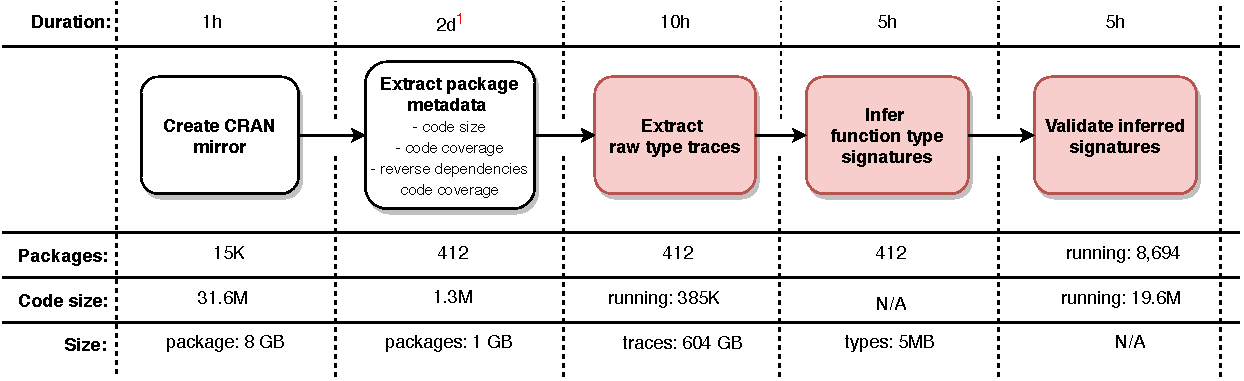
\includegraphics[width=\textwidth]{plots/analysis-pipeline-new.pdf}
  \caption{The Analysis Pipeline; $^1$ metadata has to be extracted
    for \emph{all} CRAN packages.}\label{fig:pipeline}
\end{figure}

\subsection{Types from traces}

We implemented \typetracer, an automated tool for extracting types
from execution traces of R programs. The goal of this tool is to
output a tuple $\langle f, t_1, \dots, t_n, t\rangle$ for each
function call during the execution of a program, where $f$ is an
identifier for a function, $t_i$ are type-level summaries of the
arguments and $t$ is a summary of the return value.

While seemingly simple, the details and their proverbial devil are
surprisingly tricky to get right at scale.  Our implementation reuses
\rdt, an open source dynamic analysis framework for R~\cite{oopsla19}
which consists of an instrumented R Virtual Machine based on GNU-R
version 3.5.0. The framework exposes hooks in the interpreter to which
user defined callbacks can be attached. These hooks include function
entry and exit, method dispatch for the S3 and S4 object systems, the
longjumps used by the interpreter to implement non-local exit,
creation and forcing of promises, variable definition, value creation,
mutation and garbage collection.

\paragraph{Types}
The type information output by the tool includes the \emph{type tag}
of each value. Internal types are translated to names in the proposed
type system. The next bit of information is the \emph{class}, an
optional list of names that may be absent, and, in some cases, is
implicit (i.e. the interpreter blesses some values with the \k{matrix}
and \k{array} classes even without attributes).  Depending on a
value's type, the tool collects further information: (a) for vectors,
the presence of \NA values, (b) for lists, element types by a
recursive traversal, and (c) for promises, an approximation of the
expression type.  To obtain these types, we make use of R's C FFI and
use low-level machinery to collect information from the R run-time.
Types are completed during post-processing, and rely on the detailed
information made available by these reflection mechanisms.

\paragraph{Promises}
The fact that arguments are lazy (expressions are packed into promises
and only evaluated on first access) complicates information gathering.
For example, some promises may remain unevaluated, and it would be
erroneous to force them as they may side-effect and change program
behavior.  To deal with unevaluated arguments, we make an initial
guess for each argument at function entry and update the recorded type
if the promise is forced.

\paragraph{Missing arguments}
Parameters which receive no values when the function is called are
termed missing (not to be confused with \NA). This occurs when a
function is called with too few arguments and no default values are
specified for those missing arguments.  We record a \k{missing} type
for such argument.  There are two obvious ways to deal with missing
arguments: type them as \any or type them as some unit type.  We
conservatively type them as \any.

\paragraph{Non-local returns}
When a function exits with a longjump, there is no return value to speak
of. To ensure call traces are valid when a longjump occurs, we intercept the
unwinding process and record a special \k{jumped} return type for function
returns that are skipped. As we cannot be sure of the intended return value, 
these \k{jumped} values become \any types.

\paragraph{Dots}
Arguments that are part of a dots parameter (denoted \VARGS) are
ignored. We do not attempt to give dots a type.

\paragraph{Implementation details.}
We primarily rely on eight callbacks: \k{closure\_entry},
\k{closure\_exit}, \k{builtin\_entry}, \k{builtin\_exit},
\k{special\_entry}, \k{special\_exit}, \k{promise\_force\_entry}, and
finally \k{promise\_force\_exit}.  The function-related callbacks are
used mainly for bookkeeping: the analysis is notified that a construct
has been entered by pushing the call onto a stack.  The calls
themselves store a trace object that holds the type information. As R
can perform single or multiple dispatch on function arguments
depending on their class, the relevant information is kept by the {\tt
  \_entry} variants.


\subsection{Checking signatures with contracts}

One can validate a function's type signature by checking that it is
respected in all programs that call the function.  For this, we
developed \contractr, an R package that decorates functions with
assertions. We use it to insert type checking code around functions.
For speed, \contractr's primary logic is implemented in C++.  It has
been tested with GNU R-3.5.0 and hardened with a battery of 400 test
cases.  An invocation of \code{library(contractr)} causes contracts to
be injected. \contractr scans all packages in the workspace and
inserts contracts in functions for which type signatures are
available. Package load hooks are executed when new packages are
loaded. \contractr automatically removes contracts from all functions
and restores them to their original state when it is unloaded. The
type signatures can be provided in an external file, thus avoiding the
need to change the source code of checked packages. Type declarations
can also be written in comments using \roxygen annotations, using the
\code{@type} tag:

\begin{lstlisting}
 #' @type <chr> => int
 #' @export
 file_size <- function(f) { ... }
\end{lstlisting}

The injected contracts check arguments with a simple tag check when
possible. Some properties require traversing data structures, such as
the absence of \NA. For union types, multiple checks may be needed, at
worst one per member of the union.  In order to retain the non-strict
semantics of R, the expression held in a promise is wrapped in a call
to the type checker, and type checking is delayed until the promise is
forced. This leads to corner cases such that the type checking of a
function may happen after that function has returned.  Return values
require care as well.  Functions return the last expression they
evaluate, thus a callback is added to the exit hook.  Another wrinkle
is due to longjumps which causes active function calls on the stack to
be discarded. When they are discarded, their exit hooks are called but
they do not have a return value to type-check. \contractr deals with
this problem by allocating a unique sentinel object which serves as
the return value for calls that are discarded. The exit hook does not
call the type-checker if it see the sentinel.

%%%%%%%%%%%%%%%%%%%%%%%%%%%%%%%%%%%%%%%%%%%%%%%%%%%%%%%%%%%%%%%%%%%%%%%%%%%%%
\section{Project Corpus}\label{sec:corpus} %%%%%%%%%%%%%%%%%%%%%%%%%%%%%%%%%%

For this paper we have selected \CorpusLoadable packages consisting of
\CorpusRCodeRnd lines of R code and \CorpusNativeCodeRnd lines of native
code (C/Fortran). Figure~\ref{fig:corpus} shows these packages: the size of
the dots reflects the project's size in lines of code including both R and
native code\footnote{Lines of source code reported excludes comments and
  blank lines, counted by \emph{cloc}, \cf
  \url{https://github.com/AlDanial/cloc}}, the x-axis indicates the
expression code coverage as a percentage and the y-axis gives the number of
reverse dependencies in on log scale. Dotted lines indicate means. Packages
with over \PackageSizeOutierRnd lines of code are annotated.

\begin{figure}[!h]\centering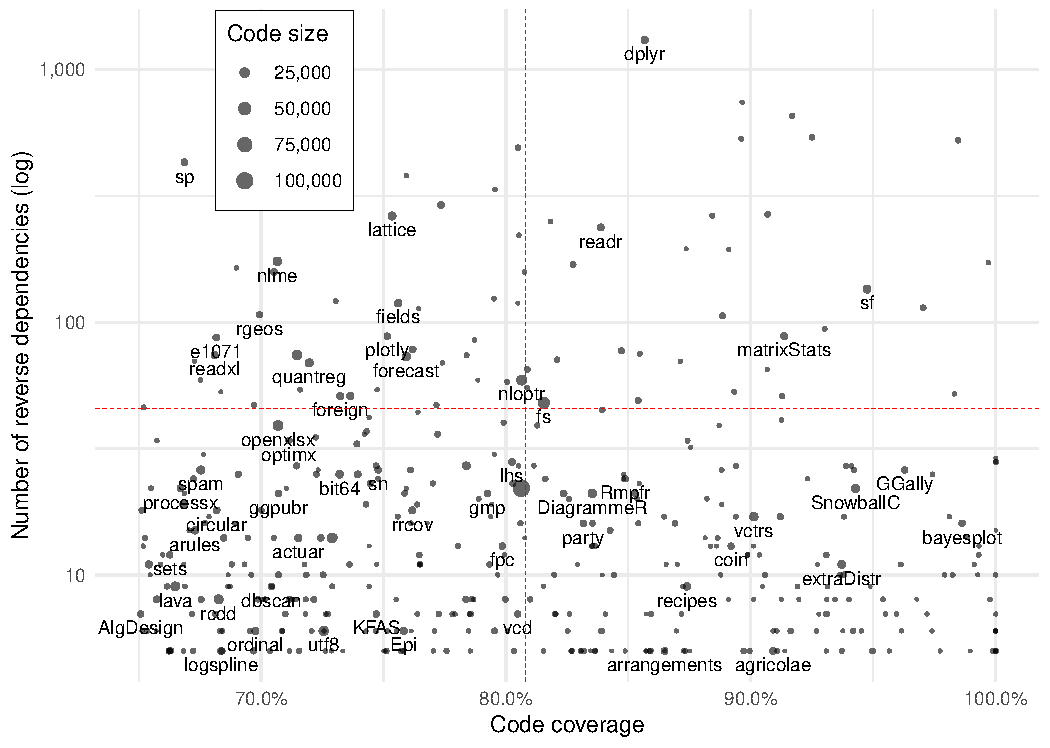
\includegraphics[width=.8\linewidth]
  {plots/corpus.pdf}\caption{Corpus}\label{fig:corpus}
\end{figure}

These packages come from the Comprehensive R Archive Network
(CRAN\footnote{\url{http://cran.r-project.org}}), the largest
repository of R code with over \AllCranRnd packages\footnote{CRAN
receives about 6 new package submissions a day~\cite{Ligges2017}}
containing over \AllRCodeRnd and \AllNativeCodeRnd lines of R and
native code respectively. Unlike other open code repositories such as
GitHub, CRAN is a curated repository where each submitted package must
abide by a number of well-formedness rules that are automatically
checked to assess package quality.  Notably, CRAN packages must have a
set of {\it runnable} example, test, and vignette code which showcase
package functionality.  The code is run by CRAN, and only a
successfully running package is admitted to the archive.

We have downloaded and installed all available CRAN packages. Out of
the \AllCranRnd packages, we managed to install \AllLoadableRnd. The
main reason for this is that \rdt (and, by extension, \typetracer) is
based on GNU-R 3.5.0 and some of the packages are not compatible with
this version.  Some packages also require extra native dependencies
which were not present on our servers. We defined two criteria for
including a package into the corpus:
\begin{inparaenum}[(1)]
  \item the package must have a runnable code that covers a
    significant part of the package source code from which type
    signatures could be inferred, and
  \item the package must have some reverse dependencies that will
    allows us to evaluate the inferred types using the runnable code
    from these dependencies.
\end{inparaenum}
The concrete thresholds used were: at least \ThresholdCodeCoverage of
expression coverage and at minimum \ThresholdRevdeps reverse
dependencies. The code coverage was computed for each package using
\covr\footnote{\url{https://github.com/r-lib/covr}}, the R code
coverage R tool.  The reverse package dependencies were extracted from
the package metadata using built-in functions.

The \CorpusLoadable selected packages contain \CorpusRunnableCodeRnd
lines of runnable code in examples (\CorpusExamplesCodeRnd), tests
(\CorpusTestsCodeRnd) and vignettes (\CorpusVignettesCodeRnd). Running
this code results on average in \CorpusMeanExprCoverage package code
coverage (the average for all of CRAN is
\AllMeanExprCoverage). Together, there is \CorpusRevdesRnd (on average
\CorpusMeanRevdes, median \CorpusMedianRevdes; CRAN average is
\AllMeanRevdes, median \AllMedianRevdes) reverse dependencies with
\CorpusRevdepRunnableCodeRnd runnable lines of code resulting in
\CorpusRevdepMeanCodeCoverage coverage (on average) of the corpus
packages.  Together there are \CorpusFunctionsRnd defined R functions
(\CorpusPublicFunctionsRnd are from the packages' public APIs).
\CorpusSThreeFunctionsRnd are S3 functions, either S3 generics or S3
methods. Packages in the corpus define \CorpusSThreeClasses S3
classes.

\paragraph{User code}%%%%%%%%%%%%%%%%%%%%%%%%%%%%%%%%%%
To represent end-user code in the corpus, we turned to Kaggle, an
online platform for data-science and machine-learning. The website
allows people to share data-science competitions and data-analysis
problems together with data for which users try to find the best
solution (something like a repository of hackathon or datathon
code). The solutions, called \emph{kernels}, are then posted on Kaggle
either as plain scripts or as notebooks. One of the most popular
competitions is about predicting passenger survival on
Titanic\footnote{\url{https://www.kaggle.com/c/titanic}} with
\KaggleDownloaded kernels in R (over 1/4 of all available R kernels)
which we used for our corpus.

Unlike CRAN, Kaggle is not a curated repository and therefore there
are no guarantees about the quality of the code. After downloading all
of the \KaggleDownloaded kernels and extracting the R code from the
various formats,\footnote{We use {\sf rmarkdown} to convert from
notebooks to R.} we found that \KaggleDuplicated were whole-file
duplicates (\KaggleDuplicatedRatio). From the resulting
\KaggleRunnable kernels, \KaggleFail failed to execute. Next to
various runtime exceptions, common problems were missing libraries (no
longer available for R 3.5), parse errors and misspelled package
names. The final set contains \KaggleSuccess kernels with
\KaggleSuccessCodeRnd lines of R code. The Kaggle kernels are used for
additional validation of the inferred types.


\paragraph{Type usage}%%%%%%%%%%%%%%%%%%%%%%%%%%%%%%%%%%
During execution 3,147 different types were observed.  Classes are the
most common types, accounting for roughly 31\% of types of arguments.
The most common classes are \c{matrices} (12\%), \c{data.frames}
(7.5\%), \c{formulas} (2\%), \c{factors} (2\%), and \c{tibbles} (2\%).
Roughly 25\% of classes are part of R's base libraries, the others are
user-defined.  Scalars and vectors are the next most common kind,
making up 41\% of remaining types. with scalars making up 28\% of
types and vectors 12\%.  Nulls and lists follow at 8\% and 7\%
respectively, and the vararg type makes up 6\% of arguments.  This all
totals up to over 90\% of types.  Table~\ref{ctb} reports on the 10
most frequent types occurring in the corpus. The first row of the
table reads: the \dbl type occurs in 12,298 (11.24\%) argument types,
and accounts for over 12 million (20.3\%) of the types observed by
\typetracer's dynamic analysis.

\begin{table}[!h]
% BEGIN Autogenerated
\small\begin{tabular}{lrrrr}\toprule
Type & Args & \% of Args & Observations & \% of Obs.\\\midrule
\dbl               & 12,298 &     11.24 &  12,152,787 & 20.3 \\
\lgl               & 9,366 &      8.7 & 6,650,294 & 11.1 \\
\nul              &  8,799 &      8.0 & 2,187,611 & 3.7 \\
\chr               &  8,727 &      8.0 & 2,564,207 & 4.3 \\
\VEC\dbl           &  7,190 &      6.6 &  4,934,773 & 8.2 \\
\VARGS             &  6,611 &      6.0 &  6,075,874 & 10.1 \\
\any               &  6,120 &      5.6 & 339,299 & 0.6 \\
\VEC\chr           &  4,325 &      4.0 &  1,060,466 & 1.8 \\
\CLASS{\texttt{matrix}}     & 4,152 & 3.8 & 2,805,718 & 4.7 \\
\CLASS{\texttt{data.frame}} & 2,608 & 2.4 &  352,655 & 0.6 \\
\bottomrule
\end{tabular}
\caption{Top types of arguments in R}\label{ctb}
\end{table}


%%%%%%%%%%%%%%%%%%%%%%%%%%%%%%%%%%%%%%%%%%%%%%%%%%%%%%%%%%%%%%%%%%%%%%%%%%%%%%
\section{Evaluation} %%%%%%%%%%%%%%%%%%%%%%%%%%%%%%%%%%%%%%%%%%%%%%%%%%%%%%%%%

We ran \typetracer on the test, example, and vignette code of the
aforementioned corpus of \PACKAGES packages and successfully inferred
types for \NUMFUNCTIONS functions.  Table~\ref{tbl:typesig}
illustrates the process with ten representative signatures.  Many of
the features of our type language are represented here, and some
signatures are telling of the function's behaviour.  For example,
consider \code{decrypt_envelope}: the first three parameters of the
function are byte arrays, and the fourth argument is an RSA key, used
to decrypt some of the inputs, and the output of the function is
another byte array.  As another example, consider \code{Traverse}:
according to the function documentation, it takes the root of a tree
and traverses it in an order specified by the second argument.  We see
that reflected in the type, where the first argument has type
\CLASS{\texttt{Node}, \texttt{R6}} and the second argument had type
\VEC\chr, representing the traversal order.

\begin{table}[H]
  \centering
  \resizebox{.98\linewidth}{!}{
  \begin{tabular}{llrrr}
    \toprule
    Function & Type Signature \\
    \midrule
    \code{dplyr::group_indices} & \FUN{\CLASS{\texttt{data.frame}}, \VARGS}{\VEC\int}\\
    \code{moments::all.cumulants} & \FUN{\CLASS{\texttt{matrix}} \; | \; \VEC\dbl}{\CLASS{\texttt{matrix}}\; | \; \VEC{\dbl}}\\
    \code{diptest::dip}& \FUN{\VEC\dbl, \chr \; | \; \lgl, \lgl,
                         \dbl}{\CLASS{\texttt{dip}} \; | \; \dbl} \\
    \code{stabledist::cospi2}& \FUN{\VEC\dbl}{\VEC\dbl} \\
    \code{matrixcalc::matrix.power}& \FUN{\CLASS{\texttt{matrix}},
                                     \dbl}{\CLASS{\texttt{matrix}}} \\
    \code{data.tree::Traverse}& \FUN{\CLASS{\texttt{Node}, \texttt{R6}}, ~\VEC\chr,
                                \any, \any}{\LIST{\any}} \\
    \code{openssl::decrypt\_envelope}& \FUN{~\VEC\raw, ~\VEC\raw, ~\VEC\raw,
                                       \CLASS{\texttt{key}, \texttt{rsa}}, \any}{\VEC\raw} \\
    \code{dbplyr::set\_win\_current\_group}& \FUN{? ~\VEC\chr}{\; ? \; \VEC\chr} \\
    \code{openssl::sha256}& \FUN{~\VEC\raw, ? ~\VEC\raw}{\VEC\raw} \\
    \code{forecast::initparam}& \FUN{? \dbl, \any, \any, \any, \chr, \chr, \lgl,
                                ~\VEC\dbl, ~\VEC\dbl, \any}{\VEC\dbl} \\
    \bottomrule
  \end{tabular}}
\caption{Select Type Signatures}\label{tbl:typesig}
\end{table}


This section attempts to evaluate how well the proposed type system is able
to describe the actual type signatures of functions. For this we focus on
how often there is a single type for a particular argument; this is because
union types and \any are less accurate (and would likely require a more
refined notion of subtyping or parametric polymorphism). Then, we evaluate
how robust the inferred signatures are by checking that they remain valid
for other inputs.  Lastly, we try to see if the current proposal would be
useful to programmers by allowing them to remove ad hoc checks and providing
useful documentation.


\subsection{Expressiveness}

The first part of our evaluation attempts to shed light on how good a fit
our proposed type system is with respect to common programming patterns
occurring in widely used R libraries.

\begin{figure}[!h]  \centering
  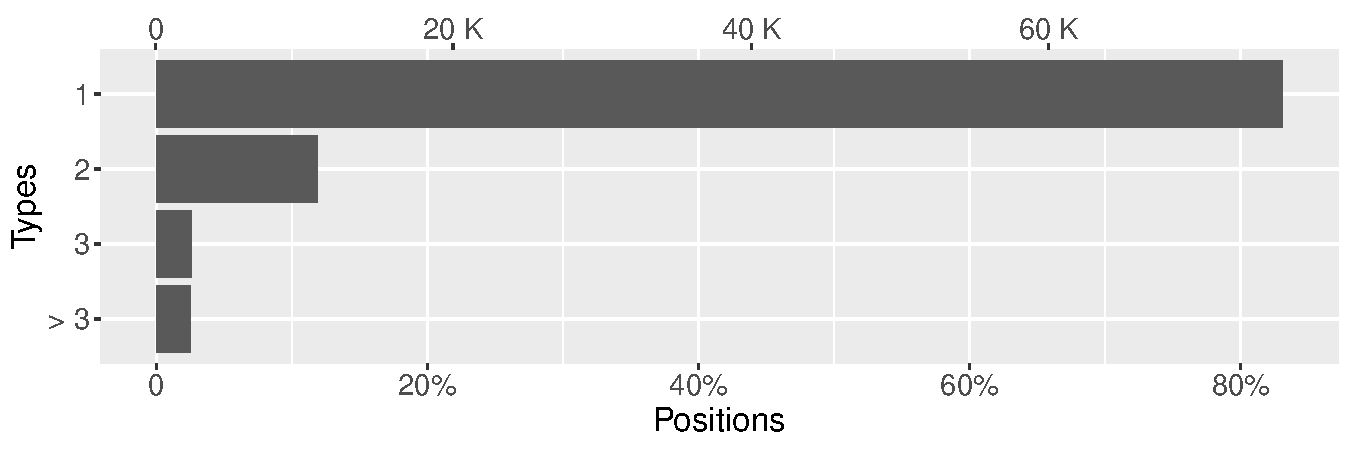
\includegraphics[width=.8\linewidth]{plots/argument_polymorphism.pdf}
  \caption{Size of unions}\label{fig:unionfreq}
\end{figure}

First we look at the share of monomorphic arguments and function signatures.
Monomorphic in this context means that the type is not relying on \any or
including a union.  The import of monomorphism in this context is that it
means our type language can accurately capture an argument's type or a
function signature. We get to that number in two steps.
Fig.~\ref{fig:unionfreq} shows the number of inferred argument types and
their size (in terms of members of the union). The figure shows the most
functions do not require a union at all (\PercUnitypedPositions of arguments
do not have a union), and only \PercManytypedPositions positions have unions
with more than three members.


\begin{table}[H]
  \centering
  \resizebox{.5\linewidth}{!}{
    \begin{tabular}{lrrr}
      \toprule
      Types & Parameter \# & \% & Cumulative \%\\
      \midrule
      scalar & 35064 & 33.33 & 33.33 \\
      class & 24256 & 23.06 & 56.39 \\
      vector & 13025 & 12.38 & 68.77 \\
      \rowcolor{lightgray}  \textcolor{black}{...} & \textcolor{black}{9142} & \textcolor{black}{8.69} & \textcolor{black}{77.46}\\
      \rowcolor{lightgray} \textcolor{black}{null} & \textcolor{black}{7694} & \textcolor{black}{7.31} & \textcolor{black}{84.77}\\
        \addlinespace
   \rowcolor{lightgray}  \textcolor{black}{any} & \textcolor{black}{7614} & \textcolor{black}{7.24} & \textcolor{black}{92.01}\\
      \rowcolor{lightgray}  \textcolor{black}{list} & \textcolor{black}{3558} & \textcolor{black}{3.38} & \textcolor{black}{95.39}\\
      \textasciicircum{}vector & 2923 & 2.78 & 98.17\\
      function & 1427 & 1.36 & 99.52 \\
      environment & 500 & 0.48 & 100.00\\
      \bottomrule
    \end{tabular}}
  \caption{Singleton Type Categories}\label{fig:singlefreq}
\end{table}

Table~\ref{fig:singlefreq} provides a breakdown of types occurring in
arguments without a union. Scalar, class and vector are the most
common type categories. The shaded rows correspond to polymorphic
types.  When an argument's type is \nul, we say that the argument is
polymorphic due to a limitation in our analysis: In R, it is common
for programmers to include default values for arguments, and in many
cases this value happens to be {\tt NULL}.  Our type analysis will
report a {\tt null} type for these arguments if they are {\it never
  passed a value} during testing.  We interpret these instances of
\nul as polymorphic to capture that we cannot be sure of the actual
type.

Removing the aforementioned instances of polymorphism gives us
\CountMonomorphicPositions (\PercMonomorphicPositions) monomorphic
positions in a corpus of \CountPositions parameters. With close to
60\% of monomorphic argument or return values, it is fair to say that
even a simple type language provides significant benefits.

\begin{figure}[!h]  \centering
  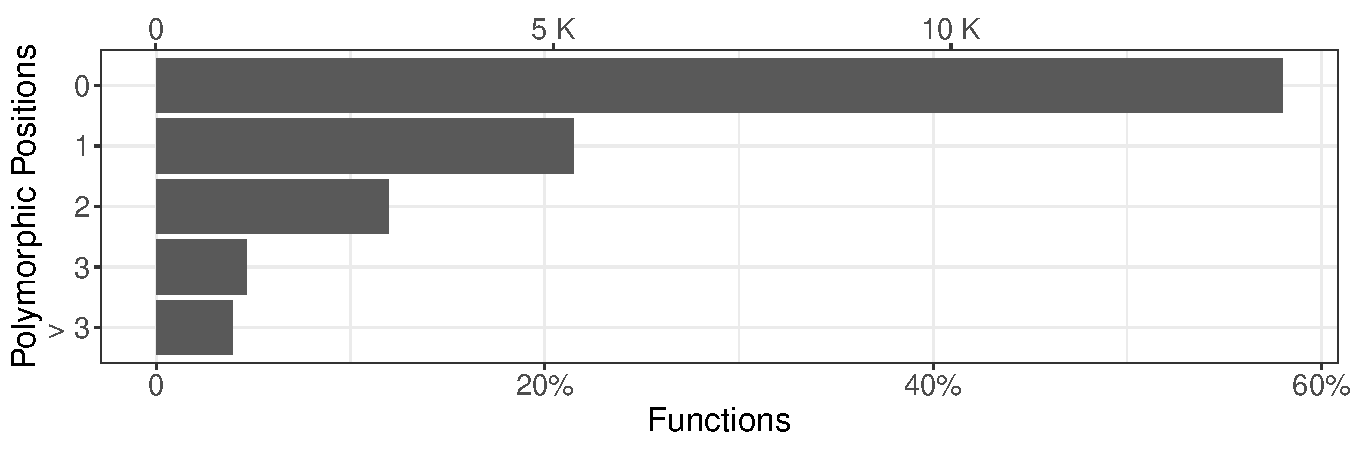
\includegraphics[width=.8\linewidth]{plots/function_polymorphism.pdf}
  \caption{Function Polymorphism}\label{fig:funpoly}
\end{figure}

If we look at the numbers from the point of view of functions and
count how many of their arguments are polymorphic, we observe that
\PercMonomorphicFunctions (\CountMonomorphicFunctions) functions are
monomorphic. The remaining \PercPolymorphicFunctions
(\CountPolymorphicFunctions) have at least one union or polymorphic
parameter or return type.  Figure~\ref{fig:funpoly} shows the
distribution of functions against the number of polymorphic
arguments. Finally, we count that \CountMonomorphicPackages out of the
412 packages export only monomorphic functions.

\subsubsection{Discussion}
A number of lessons can be drawn from the data we have gathered.

\paragraph{NAs}
Our data supports making the presence of {\NA}s explicit. Only 2923 (or
2.78\%) of arguments are marked as possibly having {\NA}s, thus the
overwhelming majority of types appear to be {\NA}-free.  In practice,
programmers check for them and sanitize them if they are present.  Consider
the \code{binom} package for computing confidence intervals and its
\code{binom.profile} function.  This attached code snippet highlights a data
sanitization pattern: the programmer first binds the vectors into a matrix,
then finds rows where both columns are not \NA, extracts non-\NA values and
stores them into \code{x} and \code{n} respectively.

\begin{lstlisting}[basicstyle=\footnotesize\ttfamily]
  binom.profile <- function(x, n, conf.level=0.9, maxsteps=50, ...) {
    xn <- cbind(x = x, n = n)
    ok <- !is.na(xn[, 1]) & !is.na(xn[, 2])
    x <- xn[ok, "x"]
    n <- xn[ok, "n"]
    # ...
  }
\end{lstlisting}

\paragraph{Scalars}
The data also suggests that programmers often use scalars, and do
dimensionality checks on their data.  In our data 25,064 (or 33.33\%) of the
arguments are scalar types. While not completely surprising, this is a
rather large number. Consider the \code{hankel.matrix} function, it takes
two arguments and checks that \code{n} is \int, that \code{x} is a vector,
and also, indirectly, that \code{n} is a a scalar (this comes from the fact
that it is used in the guard of a conditional which fails if \code{n} is
not a scalar).

\begin{lstlisting}[basicstyle=\footnotesize\ttfamily] 
  hankel.matrix <- function( n, x ) { 
    ### n = a positive integer value for the order of the Hankel matrix
    ### x = an order 2 * n + 1 vector of numeric values
    if ( n != trunc( n ) )  stop( "argument n ix not an integer" )
    if ( !is.vector( x ) )  stop( "argument x is not a vector" )
    m <- length( x )
    if ( m < n )  stop( "length of argument x is less than n" )
    # ...
  }
\end{lstlisting}

\paragraph{Nullables}
The number of argument which may be \c{NULL} is 5057 (or 4.44\%). This is a
relatively small number of occurrences, but it is worth expressing the
potential for the presence of \c{NULL} as these would likely inhibit
optimizations.

\paragraph{Higher-Order Functions}
\typetracer assigns the type \CLASS{\texttt{function}} to function
values.  The number of positions that receive a function (possibly as
part of a union) is 1,705, which is just 1.51\% of all the positions
for which we infer types. Given the small number of occurrences, it is
not worth complicating the inferred types with a complete signature
for these functions.

\paragraph{Structs}
While experimenting with various design, we consider adding a struct
type to capture lists with named elements that can be accessed with
the \code{$} operators. We ended up discarding those types as they
grew large and were often only representative of the example data
being manipulated.  Consider function \code{cv.model}, its argument
\code{x} is observed to be of \CLASS{\texttt{aov}, \texttt{lm}} or
\CLASS{\texttt{lm}}.  Internally, linear models are represented as
lists with named elements.  The pollution is illustrated by the lines
after the function definition.  They load an example data set and test
the function \code{cv.model}.  The \code{data(sweetpotato)} expression
loads a sample data set. The fields of \code{sweetpotato} will be
recorded when \code{cv.model} is called.

\begin{lstlisting}[basicstyle=\footnotesize\ttfamily]
  cv.model <- function(x) {
    suma2 <- sum(x$residual^2)
    gl <- x$df.residual
    promedio <- mean(x$fitted.values)
    return(sqrt(suma2/gl)*100/promedio)
  }
  
  data(sweetpotato)
  model<-aov(yield~virus, data=sweetpotato)
  cv.model(model)
\end{lstlisting}


\paragraph{Objects}
While we record classes, our analysis does not deal with method
dispatch.  R has multiple disparate object systems called S3, S4, and
R5.  The \code{class} attribute is used by these systems to dispatch
methods. S3 does single dispatch, S4 does multiple dispatch and R5
supports imperative objects.  The mechanics of S4 dispatch are more
complex than for S3, and users can define their own class hierarchies
that we would need to incorporate in our type analysis and contract
checking frameworks.  We found limited use of S4 during our
analysis. Coming up with a type system that accounts for all of these
factors and consolidates multiple object-orientation frameworks in a
single language design is an interesting problem in and of itself, one
we leave for future work.

\paragraph{Matrices}
Matrices are instances of the eponymous class, representing 10.71\% of
all classes occurring in types. They have a \code{dims} attribute
indicating dimensions, and while not codified in the language
semantics, many internal functions coerce vectors to matrices
automatically.  For example, the \code{rowWeightedMeans} function
calculates the weighted means of rows.  The programmer added a type
check for \code{x}.

\begin{lstlisting}[basicstyle=\footnotesize\ttfamily]
  rowWeightedMeans <- function(x, w=NULL, rows=NULL, cols=NULL, na.rm=FALSE, ...) {
    if (!is.matrix(x))   .Defunct(msg = sprintf("'x' should be a matrix.)
    # ...
  }
\end{lstlisting}


\paragraph{Data Frames}
One of the most popular classes in R is the \code{data.frame} class,
making up 8.15\% of observed classes.  Data frames and the derivative
\code{tibble} and \code{data.table} types underpin much of the
idiomatic usage of R.  One way to deal with data frames is through the
struct type, with a named field for each column of the data frame, but
as mentioned previously structs introduced undue noise.  Further
complicating data frames is that many functions built to operate on
them operate in a name-agnostic way.  For instance, the
\code{tidyverse} package ecosystem allows programmers to pass column
names to functions which operate on their data frames.  In base R,
typical data frame use is to use string column names to select rows
from the frame (unless only a single column is of interest, wherein
the \code{$} syntax is appropriate).  In sum, data frames are a
popular class of R values, and have spawned many derivative data
types, such as tibbles and data tables.  We include a \CLASS{{\tt
    data.frame}} type to cover most use-cases, and we leave a richer
type for future work on a full fledged object-oriented type system.

\subsection{Robustness}

We now ask {\it how robust are the inferred types}? To measure this,
we conducted another large-scale experiment: for each package in the
corpus, using the inferred type signatures as contracts we ran all of
the CRAN reverse dependencies for that package. In total we ran
\NUMPKGSEVAL unique packages and recorded \NUMASSERTIONS total
assertions. Overall, we found that only \PERCFAILEDASSERTIONSWUNDEF of
contract assertions failed. The limit on number of arguments (we
record only 20) accounted for \PERCASSERTIONSUNDEF failed
assertions. We found that \PERCSUCCARG of parameter types and
\PERCSUCCFUNS of function types never failed. The number of immaculate
function types increases to \PERCSUCCFUNNOSTHREE if we discount S3
object method dispatch. Overall, these numbers are promising, and
suggest that the type signatures are indeed robust.

We break down the failed assertions by type in
Table~\ref{tbl:fail-breakdown-0}.  Accounting for 36.36\% of assertion
failures are cases where a \VEC\dbl is passed where a
\CLASS{\texttt{matrix}} is expected.  Considering these types, we
might imagine them to be compatible, as a vector is just a
one-dimensional matrix.  However, not allowing this coercion was a
deliberate design decision, as coercion of this kind is ad hoc at
best, and unfortunately not a practice codified in the language.  For
example, if the vector has length $n$, should it be a $1 \times n$ or
$n \times 1$ dimensional matrix?

In a similar vein, another popular failing assertion is checking if a
${\bf dbl}[]$ has type ${\bf int}[]$, another case of commonly
performed coercion.  We did not include these types of coercions in
our type annotation framework as programmers cannot rely on them, and
it is not always the case that the coercions are safe to perform.

The second row of the table is exemplary of a pattern where vectors
are passed when scalars are expected.  In these cases, the functions
exhibiting these assertion failures were under-tested, and can operate
just as well on vectors of values.  As an example, this failure
occurred in functions from the \code{lubridate} package which provides
date/time functionality.  Many functions, e.g., \code{date_decimal}
and \code{make_datetime} turn doubles into \CLASS{{\tt POSIXct,
    POSIXt}} (which are dates in R), and they can easily operate on
vectors of doubles, producing lists of dates.

Finally, we point out that assertion failures of, e.g., \CLASS{{\tt
    data.frame}} values being passed to \CLASS{{\tt data.frame, tbl,
    tbl\_df}} arguments and \CLASS{{\tt xml\_node}} values being
passed to an argument expecting other XML-like classes are related to
our simplified take on class types.  Our type system does not encode
user-defined subtyping and coercion, which could help address these
mismatches.

\begin{table}
% BEGIN Autogenerated
\scriptsize
\begin{tabular}{llrrr}
\toprule
Passed & Arg Type & Occurrences & \% Total & Cumul. \%\\
\midrule
\VEC\dbl & \CLASS{\texttt{matrix}} & 705,036 & 36.36 & 36.36 \\ 
\VEC\dbl & \dbl & 189,800 & 9.79 & 46.15 \\ 
\chr & \CLASS{\texttt{bignum}} | \VEC\raw & 100,100 & 5.16 & 51.31 \\
\CLASS{{\tt simpleError, error, condition}} & \makecell[tl]{\CLASS{{\tt data.frame}} | \CLASS{{\tt matrix}} | \\ \CLASS{{\tt randomForest}} | \VEC\dbl} & 78,197 & 4.03 & 55.34 \\ 
  \CLASS{{\tt data.frame}} & \CLASS{{\tt data.frame, tbl, tbl\_df}} & 58,809 & 3.03 & 58.37 \\ 
  \addlinespace
  \CLASS{{\tt matrix}} & \CLASS{{\tt timeSeries}} & 53,482 & 2.76 & 61.13 \\ 
 \VEC\dbl & \VEC\int & 33,350 & 1.72 & 62.85 \\ 
 \dbl & \CLASS{{\tt data.frame}} & 32261 & 1.66 & 64.52 \\ 
  \VEC\dbl & \CLASS{{\tt data.frame}} & 31361 & 1.62 & 66.13 \\ 
  \CLASS{{\tt xml\_node}} & \makecell[tl]{\CLASS{{\tt xml\_missing}} $|$ \CLASS{{\tt xml\_nodeset}} $|$ \\ \CLASS{{\tt xml\_document, xml\_node}}} & 30,330 & 1.56 & 67.70 \\ 
\bottomrule
\end{tabular}
% END Autogenerated
\caption{Top contract failures}
\label{tbl:fail-breakdown-0}
\end{table}

In addition to the number of failed contract checks, we were
interested in how many functions had a parameter where a contract
check failed, and overall we found this to be the case in
\PROPFUNSFAILEDCHECK of functions.  To subdivide this number, we
discounted functions that were performing S3 dispatch, as they exhibit
user-defined polymorphism which we do not handle.  Removing those
functions, we see that the proportion of functions with failed
contract checks falls to \PROPFUNSFAILEDCHECKNOSTHREE. These remaining
functions were under-tested, as calls to these functions represent
only \PERCCALLSBADFUNSINTESTS of recorded calls during \typetracer's
run on the core corpus to infer types.

Turning our attention now to arguments, we found that only
\PROPARGSFAILINGASSERTS of argument types failed.
Table~\ref{tbl:fail-breakdown-0} showed the runtime occurrences, but
that data alone does not tell the full story, as some failures may be
overrepresented if, e.g., a failing contract assertion was in a loop.
We were interested in knowing for each of the most common violations
in Table~\ref{tbl:fail-breakdown-0}, how many different arguments had
that type, and how many of those exhibited the contract failure in
question.  Table~\ref{tbl:fail-breakdown-1} breaks down the failed
assertions by type, folding away multiple identical failed contract
assertions for the same parameter position.  The first row of this
table reads: a value of type \VEC\dbl was passed to 15 different
function parameters expecting a \CLASS{\texttt{matrix}}, of which
there are 1522 in total: 18 (1.18\%) of these
\CLASS{\texttt{matrix}}-typed parameters were passed \VEC\dbl values.

We see that even though the double vector and matrix issue was wildly
prevalent in the raw, dynamic contract evaluation numbers, the number
of actual function argument types that were violated is very small.
The story is similar with the double and integer coercion we mentioned
earlier: it represents many dynamic contract failures, but very few of
the \VEC\int-typed arguments have their contracts violated by
\VEC\dbl-typed values.  Row six is interesting: we see that rather
often arguments expecting \CLASS{\texttt{timeSeries}} data are passed
\CLASS{\texttt{matrix}} values.  This is a quirk of the
\code{timeSeries} package, whose functions often accept matrices and
vectors, converting them to time series in an ad hoc manner.  Note
that the code coverage of the \code{timeSeries} tests, examples, and
vignettes package code is only 58\%, which is one possible explanation
of why these contract failures are occurring: the types that
\typetracer generates are only as good as the test code its run on.

 \begin{table}
% BEGIN Autogenerated
\scriptsize
\begin{tabular}{llrrr}
\toprule
              &                &      \multicolumn{2}{c}{\# Args Types}        &  \\
 Passed & Arg Type & Failed & Total & \% Failure\\
\midrule
\VEC\dbl & \CLASS{\texttt{matrix}} & 18 & 1522 & 1.18 \\ 
\VEC\dbl & \dbl  & 66 & 5865 & 1.13 \\ 
\chr & \CLASS{\texttt{bignum}} | \VEC\raw & 1 & 3 & 33.33 \\ 
\CLASS{{\tt simpleError, error, condition}} & \makecell[tl]{\CLASS{{\tt data.frame}} | \CLASS{{\tt matrix}} | \\ \CLASS{{\tt randomForest}} | \VEC\dbl}  & 2 & 2 & 100 \\ 
  \CLASS{{\tt data.frame}} & \CLASS{{\tt data.frame, tbl, tbl\_df}} & 23 & 196 & 11.73 \\ 
  \addlinespace
  \CLASS{{\tt matrix}} & \CLASS{{\tt timeSeries}} & 21 & 39 & 53.85 \\ 
 \VEC\dbl & \VEC\int & 31 & 624 & 4.97 \\ 
 \dbl & \CLASS{{\tt data.frame}} & 2 & 1025 & 0.20 \\ 
  \VEC\dbl & \CLASS{{\tt data.frame}}  & 6 & 1025 & 0.59 \\ 
  \CLASS{{\tt xml\_node}} & \makecell[tl]{\CLASS{{\tt xml\_missing}} $|$ \CLASS{{\tt xml\_nodeset}} $|$ \\ \CLASS{{\tt xml\_document, xml\_node}}}   & 1 & 1 & 100 \\ 
\bottomrule
\end{tabular}

% END Autogenerated
 \caption{Results from Table 4, broken down by occurrences of the expected type as a parameter type}
 \label{tbl:fail-breakdown-1}
 \end{table}

Table~\ref{tbl:fail-breakdown-2} presents data on the most frequently
violated contracts amongst the most frequently occurring argument
types.  We selected argument types which were in the 90th percentile
of argument type occurrences, computed the most frequent type
signature violations among them, and reported the most frequently
violated contracts together with the type of the value that violated
that contract.  The first row of the table reads: 31 function
arguments with \VEC\int type are passed \VEC\dbl values instead, and
624 arguments have \VEC\int type, representing a failure rate of
4.97\%.

Had we failed to capture some key usage pattern of R with our type
annotation framework, we would likely see it here, and we can see this
in action if we consider Table~\ref{tbl:fail-breakdown-3}, which was
obtained identically to Table~\ref{tbl:fail-breakdown-2} except
selecting arguments in the 80th percentile instead.  The most frequent
argument type violation pattern in that of \CLASS{{\tt matrix}},
\VEC\dbl, and \CLASS{\texttt{data.frame}} values passed to arguments
expecting \CLASS{{\tt timeSeries}}.  This occurs in 35.90\% of such
arguments, and represents cases where tests did not adequately cover
all valid function inputs.  Separate from the issue of testing, we can
capture this behaviour with user-defined subtyping or coercion, as the
data types which were passed are readily convertible to \CLASS{{\tt
    timeSeries}}.

 \begin{table}
% BEGIN Autogenerated\
\scriptsize
\begin{tabular}{llrrr}
\toprule
Passed & Arg Type & \# Args Failed & \# Args with Type & \% Failure\\
\midrule
\VEC\dbl & \VEC\int & 31 & 624 & 4.97 \\
\dbl & \int & 21 & 519 & 4.05\\
\VEC\chr & \chr | \nul & 10 & 256 & 3.91 \\
\NAVEC\lgl & \VEC\lgl & 8  & 219 & 3.65 \\
\NASCA\lgl & \VEC\lgl & 5 & 219 & 2.28 \\
\bottomrule
\end{tabular}
% END Autogenerated
 \caption{Highest failure rate among popular argument types, for
   argument signatures whose frequency is in the 90th percentile.}
 \label{tbl:fail-breakdown-2}
 \end{table}
 
  \begin{table}
% BEGIN Autogenerated
\scriptsize
\begin{tabular}{ll@{}rrr@{}}
\toprule
Passed & Arg Type & \#Args Fail & \#Args w Type & \% Failure\\
\midrule
\CLASS{{\tt matrix}} & \CLASS{{\tt timeSeries}} & 21 & 39 & 35.90 \\
\VEC\dbl & \CLASS{{\tt timeSeries}} & 21 & 39 & 35.90 \\
\CLASS{{\tt data.frame}} & \CLASS{{\tt timeSeries}} & 14 & 39 & 35.90 \\
\CLASS{{\tt dtplyr\_step\_first, dtplyr\_step}} & \makecell[tl]{\CLASS{{\tt data.frame}} | \\ \CLASS{{\tt data.frame, grouped\_df, tbl, tbl\_df}} | \\ \CLASS{{\tt data.frame, tbl, tbl\_df}}} & 10 & 45 & 22.22 \\
\chr & \raw & 6 & 31 & 19.35 \\
% \CLASS{\texttt{data.frame}} & \CLASS{\texttt{data.frame}, \texttt{tbl}, \texttt{tbl\_df}} & 63 & 284 & 22.18\\
% \CLASS{\texttt{matrix}} & \CLASS{\texttt{array}} & 13 & 70 & 18.57\\
% \NAVEC\lgl & \lgl | \nul & 9 & 49 & 18.37\\
% \VEC\chr & \LIST{\VEC\chr} & 20 & 109 & 18.35\\
% \VEC\clx & \clx & 7 & 42 & 16.67\\
\bottomrule
\end{tabular}
% END Autogenerated
 \caption{Highest failure rate among popular argument types, for argument signatures whose frequency is in the 80th percentile.}
 % *: Grouped Tibble is \CLASS{{\tt data.frame, grouped\_df, tbl, tbl\_df}} , and Tibble is \CLASS{{\tt data.frame, grouped\_df, tbl, tbl\_df}}.}
 \label{tbl:fail-breakdown-3}
 \end{table}
 
In sum, we believe that this evaluation shows that the type signatures we
generate from traces are quite good.  Only \PERCFAILEDASSERTIONSWUNDEF of
contract assertions failed at runtime, representing failures in as few as
\PROPARGSFAILINGASSERTS of argument types.  Even though
\PROPFUNSFAILEDCHECKNOSTHREE of functions had at least one argument type
involved in a failing contract check, these functions are under-tested,
representing only \PERCCALLSBADFUNSINTESTS of calls observed while inferring
types. 

\pagebreak

 %
 %
 \subsubsection{Other Observations}
 
 We drew a number of other observations from the contract assertion
 failure data.
 
 First, we were curious about how many \nul-typed values flowed into
 non-nullable arguments, and we found that they accounted for
 \NUMNULLASSERTERRORS of contract assertion failures in
 \NUMFUNSWITHNULLASSERTERROR functions.  We manually inspected some of
 the offending functions and observed three main patterns.
 
 First, we found that many of these errors occurred in arguments that
 have a {\tt NULL} default value.  This would be the case when the
 programmer only tested the function by passing values to these
 null-by-default arguments, and clients of the package make use of the
 default.  As an example, we observed a contract assertion failure
 when {\tt inner} and {\tt labels} were {\tt NULL} in the following
 function:
 \begin{lstlisting}
  nlme::nfGroupedData <- function (formula, data = NULL, order.groups = TRUE, 
    FUN = function(x) max(x, na.rm = TRUE), outer = NULL, inner = NULL, 
    labels = NULL, units = NULL) {
    # ...
  }
 \end{lstlisting}
 
 The other two patterns are for arguments with no default value, where
 either the call results in an error (perhaps explicitly handled by
 the programmer), or results in valid function behaviour that was
 untested by the original package designer.  Here, the first case can
 be explained by a lack of testing, and the second case is explained
 by programmers not fully understanding R's language semantics.  For
 example, we observed this kind of error in the following function:
 \begin{lstlisting}
  BBmisc::convertIntegers <- function (x) {
    if (is.integer(x)) 
        return(x)
    if (length(x) == 0L || (is.atomic(x) && all(is.na(x)))) 
        return(as.integer(x))
    # ...
  }
 \end{lstlisting}
Here, if {\tt x} is {\tt NULL}, the second branch of the conditional
will be triggered (as in R, \code{length(NULL) == 0}), and the
function will return \code{as.integer(NULL)}, which curiously returns
\code{integer(0)}, a zero-length vector of integers (one might expect
it to return the integer \code{NA} value, or error).

 Next, we analyzed how often vectors were passed to arguments
 expecting scalars.  We found that \PERCDYNAMICVECERRORS of dynamic
 contract assertion failures were of this type, and these errors were
 present in \NUMFUNSWITHVECASSERTERROR functions.  Besides an outright
 error, this kind of contract assertion failure might indicate that a
 function was not well-tested, in that it was only ever tested with
 unit-length vectors being passed to an argument which is intended to
 have a vector type.  Further, these errors may reveal functions that
 were not designed with a vector-typed argument in mind, but can in
 fact handle vectors of values (in R, most functions that can accept
 scalars can also accept vectors).  As an example, consider the
 function \code{BBmisc::strrepeat}, which takes a string and repeats
 it a specified number of times:
 \begin{lstlisting}
  BBmisc::strrepeat <- function (x, n, sep = "") {
    paste0(rep.int(x, n), collapse = sep)
  }

  BBmisc::strrepeat("a", 3) # => "aaa"
  BBmisc::strrepeat(c("a", "b"), 3) # => "ababab"
 \end{lstlisting}
 This function was only ever tested with unit-length vectors passed to
 {\tt x}, even though technically it can handle longer vectors, as per
 the two sample calls above.  This could be attributed to poor quality
 testing, or misunderstanding language semantics (e.g.,
 misunderstanding the semantics of \code{paste0} and \code{rep.int}),
 but we found other instances of type errors where the functions
 really ought to have been tested with the offending type, for
 instance:
 \begin{lstlisting}
combinat::permn <- function (x, fun = NULL, ...) {
    if (is.numeric(x) && length(x) == 1 && x > 0 && trunc(x) == x) 
        x <- seq(x)
    # ...
}
 \end{lstlisting}
 As per the documentation, this function is intended to take a vector,
 and generate all permutations of elements in that vector.  If given a
 scalar ``integer'' $n$, it will generate all permutations for the
 list $[1, 2, ..., n]$.  Interestingly, the function was only tested
 by passing an integer, and not ever with a vector (even though,
 presumably, that is the main utility of the function).

Finally, we were curious to see what patterns of errors occurred in
arguments expecting classes.  Overall we found that \PERCFAILASSCLASS
of assertion failures were on arguments which were expecting a class
in some way (\PERCFAILEDONECLASS of assertion failures were on
monomorphic arguments expecting a class, the remainder on polymorphic
arguments with at least one option being a class).

There are two broad divisions which account for most of the
class-related contract assertion failures that are not outright
errors.  First, we observe a class of errors related to classes being
passed to arguments expecting a different, yet convertible class.  For
instance, we observed \CLASS{{\tt data.frame}} values being passed to
arguments expecting tibbles or data.tables (data frames have a
straightforward conversion to these classes).  Second, we observe a
class of errors related more to coercion between simple data types and
classes.  As an example, consider the aforementioned assertion
failures in the \code{timeSeries} package, and as a further example we
found many instances of \CLASS{{\tt matrix}}, \CLASS{{\tt
    data.frame}}, and vectors being passed to arguments expecting
\CLASS{{\tt array}}, a generalization of matrices.

 %
 %
 \subsubsection{Kaggle}

 To further validate our inferred types, we repeated the experiment
 discussed in this section on end-user R code found on the Kaggle
 competition website.
 
 By-and-large, we saw no meaningful difference in the two data sets,
 with the contract assertion failure patterns being repeated from the
 reverse dependencies.  Overall, we observed that
 \PERCFAILEDASSERTIONSKAGGLE of all contract assertions failed while
 running Kaggle code.  If we remove assertion failures related to our
 simplifying assumption that function types will not have more than 20
 arguments, that number drops to a mere
 \PERCFAILEDASSERTIONSKAGGLENOUNDEF.  In all,
 \PROPFUNSWITHFAILEDASSERTKAGGLE functions had at least one contract
 failure.  There were \NUMTOTALASSERTIONSKAGGLE assertions in total,
 on \NUMASSERTEDFUNCTIONSKAGGLE functions.
 
 \begin{table}[ht]
 \scriptsize
\centering
\begin{tabular}{llrrr}
\toprule
Passed & Arg Type & Occurrences & \% Total & Cumulative \%\\
\midrule
 \CLASS{{\tt data.table, data.frame}} & \CLASS{{\tt matrix}} & 20002 & 28.15 & 28.15 \\ 
 \CLASS{{\tt factor}} & \NAVEC\chr & 18344 & 25.81 & 53.96 \\ 
 \CLASS{{\tt factor}} & \VEC\chr  & 7519 & 10.58 & 64.54 \\ 
 \VEC\chr & \makecell[tl]{\LIST{\VEC\int} $|$ ... $|$ \\ \LIST{\CLASS{{\tt formula, quosure}}}} & 5385 & 7.58 & 72.12 \\ 
 \CLASS{{\tt ixforeach, iter}} & \makecell[tl]{\CLASS{{\tt dataframeiter, iter}} $|$ ... $|$ \\ \CLASS{{\tt iforeach, iter}}} & 4139 & 5.82 & 77.94 \\ 
\bottomrule
\end{tabular}
\caption{Top contract failures in Kaggle kernels}
\label{tbl:fail-breakdown-0-kaggle}
\end{table}
 
 \begin{table}
% BEGIN Autogenerated\
\small
\begin{tabular}{llrrr}
\toprule
Passed & Arg Type & \# Args Failed & \# Args with Type & \% Failure\\
\midrule
\VEC\chr & \chr & 12 & 304 & 0.04 \\ 
\CLASS{{\tt factor}} & \VEC\chr & 7 & 199 & 0.04 \\ 
\VEC\dbl & \VEC\chr & 6 & 199 & 0.03 \\ 
\NAVEC\chr & \VEC\chr & 4 & 199 & 0.02 \\ 
\int & \chr & 5 & 304 & 0.02 \\ 
\bottomrule
\end{tabular}
\caption{Highest failure rate among popular argument types in Kaggle, for argument signatures whose frequency is in the 90th percentile.}
 \label{tbl:fail-breakdown-2-kaggle}
\end{table}
 
 To mirror our analysis of contract assertions on the reverse
 dependencies of our corpus, we show in
 Table~\ref{tbl:fail-breakdown-0-kaggle} the most frequently failing
 contract in Kaggle.  While we don't see many overlapping entries per
 se, the assertions exhibit similar patterns.  For instance, {\it data
   tables} (which have \CLASS{{\tt data.table, data.frame}}) are often
 passed to arguments expecting a \CLASS{{\tt matrix}}.  Data tables
 are essentially serve the same purpose as data frames and tibbles.
 As it happens, data tables can be coerced to matrices if their
 elements are unityped, and programmers will often interchange the
 two, as is the case here.  One function producing many of these
 errors is the following:
 \begin{lstlisting}
class::knn <- function (train, test, cl, k = 1, l = 0, prob = FALSE, use.all = TRUE)  {
    train <- as.matrix(train)
    test <- as.matrix(test)
    ...
}
 \end{lstlisting}
 We see that \code{class::knn} coerces its first two arguments to matrices.
 On the topic of coercion, rows two and three of Table~ are interesting as they depict {\it factors} being passed to arguments expecting character vectors.
 \CLASS{{\tt factor}} typed values are known as factors in R, and they are stored as a vector of integer values corresponding to a set of character values, and their purpose is to allow for R to quickly deal with categorized data.
 Factors can be readily converted to characters when needed, as evidenced by these assertion failures.
 
 Another interesting entry in Table~\ref{tbl:fail-breakdown-0-kaggle}
 is the fifth row, where a \CLASS{{\tt ixforeach, iter}} is being
 passed to an argument expecting a long union of classes, each of the
 form \CLASS{{\tt X, iter}}.  This is likely an instance where the
 user defined their own class, {\tt ixforeach}, and wanted to use the
 \code{iterators} package (the user called \code{iterator::iter} with
 a \CLASS{{\tt ixforeach}}, and it gained the class {\tt iter} on
 return).  As we mentioned, accounting for object-orientation in the
 type system is beyond the scope of this work, and such an inclusion
 would allow us to better type situations like this.
 
 Table~\ref{tbl:fail-breakdown-2-kaggle} mirrors
 Table~\ref{tbl:fail-breakdown-2} in showing contract violations on
 the most frequently occurring argument types.  Here, our manual
 analysis has revealed similar failure patterns.  In the case of
 vectors being passed to scalars, we find functions which can take
 vectors but were only tested with scalars (e.g.,
 \code{stringr::str_to_upper} which converts a vector of characters to
 upper case, and \code{dplyr::anti_join}, which can join by a vector
 of column names but was only ever tested with a scalar).  We also see
 possibly-NA character vectors being passed to NA-free character
 vectors.  These assertion failures arise from a lack of testing: the
 offending functions are \code{str_trim}, \code{str_sub}, and
 \code{str_replace_all} from the \code{stringr} package.  These
 functions are actually wrappers for other functions which have the
 correct argument type (\NAVEC\chr).
 
 \subsubsection{Discussion}
 
 Overall, the analysis discussed in this section has revealed two
 broad categories of contract assertion failures: those related to
 coercion, and those related to a class hierarchy.  Our type system
 does not account for coercion as coercion in R is ad hoc at best, and
 it is implemented on a function-by-function basis, even in the core R
 packages.  As for errors related to a class hierarchy, we aim to
 tackle this in future work, as designing a full fledged
 object-oriented type system for a language like R is outside of the
 scope of this work.
 
%
%
%
%
\subsection{Usefulness of the Type Checking Framework}

There are a number of ways to check the types of function parameters
in R.  The default and most common way\footnote{\CranStopifnotRatio of
all runtime checks in the whole of CRAN} is to use the
\code{stopifnot} function from the R base package. It takes a number
of R expressions which all should evaluate to true otherwise a runtime
exception is thrown with a message quoting the corresponding failed
expression. For example, the following code checks whether a given
parameter \code{x} is a scalar string:
%
\begin{lstlisting}
stopifnot(is.character(x), length(x) == 1L, !is.na(x))
\end{lstlisting}

Besides \code{stopifnot}, there are 4 packages in
CRAN\footnote{Packages are available on the CRAN website:
\url{https://cran.r-project.org/web/packages/}} that focus on runtime
assertions: \emph{assertive}, \emph{ensurer}, \emph{assertr} and
\emph{assertthat}. \emph{assertive} and \emph{ensurer} have not been
updated since 2016 and 2015 respectively, and \emph{assertr} is used
by only \AssertrRevdeps other packages and currently focuses on
checking properties of data frames. Only the \emph{assertthat} package
is maintained and used (with \AssertthatRevdeps reverse
dependencies). The advantage of \emph{assertthat} over the R's default
is that it provides much better error messages.

One way to asses the usefulness of our type checking system is to find
out how many of the existing type checking constrains could be
replaced by \contractr.  To measure this, we have extracted all calls
to \code{stopifnot} and \code{assertthat} assertions and checked which
among them could be either completely replaced by \contractr or at
least partially simplified by removing a portion of an assertion
expression. This is useful, because a common pattern is that the first
part of the parameter assertion checks its type while the rest checks
its value. In the example above, the whole expression could be
replaced by a \chr type check.

Out of the \CorpusLoadable packages, \CorpusAssertsInPackages use
runtime assertions. Together there are \CorpusAsserts asserts in
\CorpusAssertsInFunctions functions. Among these, \contractr can
replace \CorpusTypedAsserts (\CorpusTypedAssertsRatio) assertion calls
across \CorpusTypedAssertsPackages packages and
\CorpusTypedAssertsFunctions functions.  Furthermore, additional
\CorpusPartiallyTypedAsserts (\CorpusPartiallyTypedAssertsRatio)
asserts in packages \CorpusPartiallyTypedAssertsPackages packages and
\CorpusPartiallyTypedAssertsFunctions functions could have been
simplified.

Checking the type of function parameters is not something that is seen
often in the R code. In the whole of CRAN, there are only
\CranAssertsRnd asserts in \CranAssertsInFunctionsRnd functions define
in \CranAssertsInPackagesRnd packages.  One may speculate that this is
the case due to the verbosity and inconvenience of the existing
assertion tools.  Our system can infer type annotations for existing
functions automatically. This can remove or partially remove over
\CorpusPartiallyTypedAssertsRatio of existing assertions.

%
%
%
%
\section{Discussion}

Throughout this paper, we employed the following strategy to consolidate types: We collected all of the traces observed for a function, and combined them into a single function type, where the type for each argument position was made up of a union of all the observed types at that position.
We then simplified these unions using the rules presented in Section~\ref{fig:siplification-rules}.
We call this an {\it arrow of unions}.
This strategy was not developed in a vacuum, and we will now discuss some of the decisions that went into it.

Arguably, the primary issue with the arrow of unions strategy is that of a loss of precision, as relationships between argument and return types are obscured when all argument and return types are unioned.
For example, consider a function with two unique call traces, \FUN{\chr}{\chr} and \FUN{\dbl}{\dbl}.
The strategy we employed results in a combined type of \FUN{\chr \;|\; \dbl}{\chr \;|\; \dbl} for the function, which obscures the (potential) relationship between the argument and return type.

One solution to this is simply to convert each call trace into an arrow type, and generate a union of arrow types as the overall type for the function, dubbed the basic {\it union of arrows} strategy.
This would lead to the type  \FUN{\chr}{\chr} $|$ \FUN{\dbl}{\dbl} for the aforementioned function.
Unfortunately, this leads to a significant blow-up in the size of types, and makes many types unreadable, due to the myriad ways in which we combine the primitive types, as recall that, e.g., scalars and vectors are not the same type, and we see many types of the form \FUN{\chr}{\dbl} $|$ \FUN{\VEC\chr}{\dbl} $|$ \FUN{\NAVEC\chr}{\dbl}.
When comparing this consolidation strategy against the one employed throughout the paper, we find that the types using this strategy are much larger, with 14,057 (55.06\%) functions have at least one top-level union. %, and that 16,745 (65.59\%) functions have two or fewer top-level alternatives. 
We observed 93,229 independent signatures using this strategy.

Another option is to employ a hybrid approach, wherein we perform the union of arrow types {\it after} grouping them together by return type (to further simplify we also combine some primitive return types together, such as \dbl and \VEC\dbl).
While this has the advantage of reducing most of the blow-up of the previous approach, it suffers particularly when functions return classes, as our type system does not allow us to effectively consolidate class types.
Comparing again to the strategy employed throughout the paper, we find 5,317 (20.82\%) functions to have a union of arrows, and 38,650 independent signatures.
Most functions only have one or two top-level alternatives (23,530, or 92.17\%).
We additionally find that 38,650 (26.14\%) of arrow types have at least one polymorphic argument.

These findings are summarized in Figure~\ref{fig:mergecomp}, which shows a breakdown of the number of {\it top-level alternatives} in the function types obtained with both of these strategies.
The term ``top-level alternative'' signifies an arrow type in the union of arrows, e.g., \FUN{\chr}{\chr} and \FUN{\dbl}{\dbl} are top-level alternatives in the type \FUN{\chr}{\chr} $|$ \FUN{\dbl}{\dbl}.
We see that the hybrid approach greatly increases the number of functions with no union of arrows at the function level, and nearly 5\% of function types obtained with the basic union of arrows strategy have over 9 top-level alternatives.

\begin{figure}[!h]  \centering
	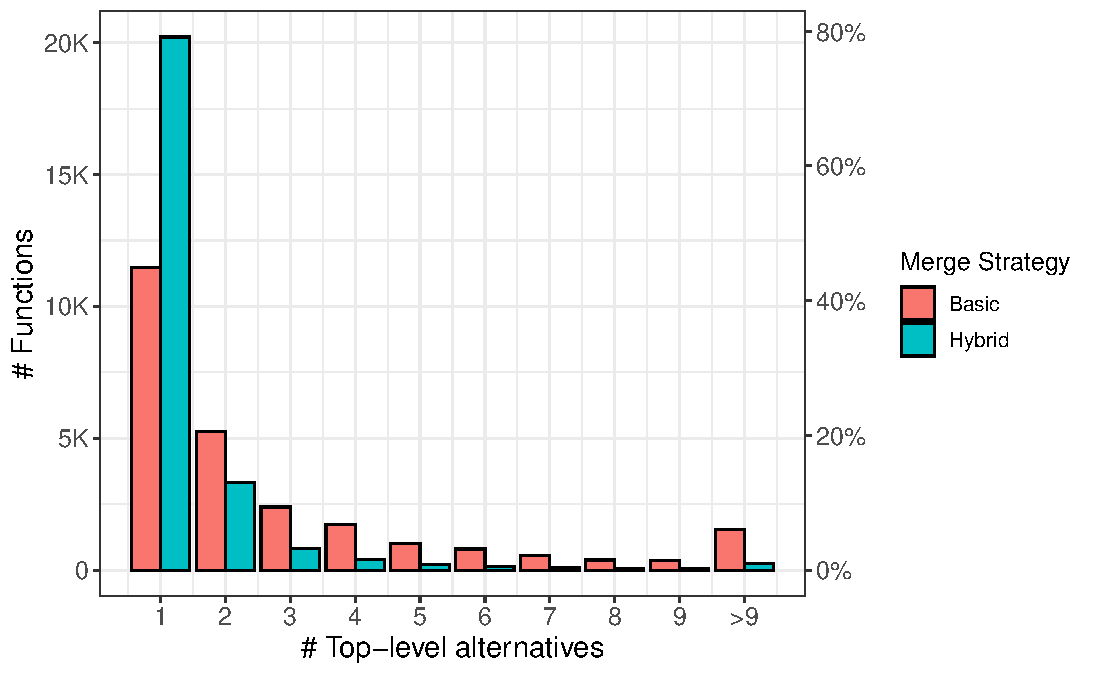
\includegraphics[width=.8\linewidth]{plots/merge_strategy_comp.pdf}
	\caption{Comparison of top-level function type counts across different merge strategies.}\label{fig:mergecomp}
\end{figure}

% To connect this discussion with actual R types, we chose the \code{discretize} function from the \code{arules} package, and show what the type of the function would be when using each of these strategies.
% The purpose of the function is to convert a continuous variable into a categorical variable, using several unsupervised learning methods.
To connect this discussion with actual R types, we chose the \code{correlation} function from the \code{agricolae} package, and show what the type of the function would be when using each of these strategies.
\code{agricolae::correlation} obtains the coefficients of correlation and p-value between all variables of some input data table, and uses a method of the user's choosing.
It returns the correlation matrix and the probability together in a list.
We refer the reader to Figure~\ref{tbl:real-function-different-merge-strats}, where we see that the hybrid approach produces a much smaller type, with only two arrow types in the top-level union.
Moreover, we see that no real precision is lost when further reducing the function type to a pure arrow of unions, as the two top-level alternatives in the type obtained with the hybrid approach are not very informative.

\begin{table}[H]
	\centering
	 \resizebox{.98\linewidth}{!}{
		\begin{tabular}{llrrr}
			\toprule
			Merge Strategy & Function Type \\
			\midrule
			Union of Arrows & \makecell[tl]{
				\FUN{\VEC{\dbl}, \VEC{\dbl}, \chr, \chr}{\nul} | \\
				\FUN{\VEC{\int}, \VEC{\dbl}, \chr, \chr}{\nul} | \\
				\FUN{\CLASS{{\tt data.frame}}, \nul, \VEC\chr, \chr}{\LIST{\CLASS{{\tt matrix}} \; | \; \dbl}} | \\
				\FUN{\CLASS{{\tt data.frame}}, \nul, \chr, \chr}{\LIST{\CLASS{{\tt matrix}} \; | \; \dbl}} | \\
				\FUN{\VEC\dbl, \CLASS{{\tt data.frame}}, \VEC\chr, \chr}{\LIST{\CLASS{{\tt matrix}} \; | \; \dbl}} | \\
				\FUN{\VEC\dbl, \CLASS{{\tt data.frame}}, \chr, \chr}{\LIST{\CLASS{{\tt matrix}} \; | \; \dbl}}
			} \\
		\addlinespace
			Hybrid & \makecell[tl]{
				\FUN{\VEC{\dbl}, \VEC{\dbl}, {\chr}, {\chr}}{\nul} | \\
				\FUN{\CLASS{{\tt data.frame}} \; | \; \VEC{\dbl}, ? \; \CLASS{{\tt data.frame}}, \VEC{\chr}, {\chr}}{\LIST{\CLASS{{\tt matrix}} \; | \; \dbl}}} \\
			\addlinespace
			Arrow of Unions & \FUN{\CLASS{{\tt data.frame}} \; | \; \VEC{\dbl}, ? \; \VEC{\dbl} \; | \; \CLASS{{\tt data.frame}}, \VEC{\chr}, {\chr}}{\, ? \; \LIST{\CLASS{{\tt matrix}} \; | \; \dbl}} \\
			\bottomrule
	\end{tabular}}
	\caption{Types of \code{agricolae::correlation} with different type merge strategies. }\label{tbl:real-function-different-merge-strats}
\end{table}

In contrast, there are real cases where a meaningful loss of precision occurs.
Consider instead the \code{rename} function from the \code{dplyr} package, with types shown in Figure~\ref{tbl:real-function-different-merge-strats-2}.
This function takes a data frame and renames selected columns.
We see that with both the union-of-arrows and hybrid approach, the types are the same (with only three unique function signatures observed), and can glean from these types that \code{dplyr::rename} produces a data frame of the {\it same class} as the input.
This information is lost in the arrow-of-unions merge strategy.
That said, once the type system is extend with proper user-defined type hierarchies, the arrow of unions type will be much smaller and more informative (as data frames, grouped tibbles, and tibbles are likely all related types).

\begin{table}[H]
	\centering
	\resizebox{.98\linewidth}{!}{
		\begin{tabular}{llrrr}
			\toprule
			Merge Strategy & Function Type \\
			\midrule
			Union of Arrows &  \makecell[tl]{
		      \FUN{\CLASS{{\tt data.frame}}, ...}{\CLASS{{\tt data.frame}}}	| \\
             \FUN{\CLASS{{\tt data.frame, grouped\_df, tbl, tbl\_df}}, ...}{\CLASS{{\tt data.frame, grouped\_df, tbl, tbl\_df}}} | \\
             \FUN{\CLASS{{\tt data.frame, tbl, tbl\_df}}, ...}{\CLASS{{\tt data.frame, tbl, tbl\_df}}}
			} \\
		\addlinespace
			Hybrid & \makecell[tl]{
				\FUN{\CLASS{{\tt data.frame}}, ...}{\CLASS{{\tt data.frame}}}	| \\
				\FUN{\CLASS{{\tt data.frame, grouped\_df, tbl, tbl\_df}}, ...}{\CLASS{{\tt data.frame, grouped\_df, tbl, tbl\_df}}} | \\
				\FUN{\CLASS{{\tt data.frame, tbl, tbl\_df}}, ...}{\CLASS{{\tt data.frame, tbl, tbl\_df}}}
			} \\
		\addlinespace
			Arrow of Unions & \makecell[tl]{
				$\langle \CLASS{{\tt data.frame}} \;|\; \CLASS{{\tt data.frame, tbl, tbl\_df}} \;|\; \CLASS{{\tt data.frame, grouped\_df, tbl, tbl\_df}}, ... \rangle$ $\rightarrow$ \\
				$\CLASS{{\tt data.frame}} \;|\; \CLASS{{\tt data.frame, tbl, tbl\_df}} \;|\; \CLASS{{\tt data.frame, grouped\_df, tbl, tbl\_df}}$
			} \\
			\bottomrule
	\end{tabular}}
	\caption{Types of \code{X::Y} with different type merge strategies. }\label{tbl:real-function-different-merge-strats-2}
\end{table}

Finally, we want to briefly discuss types for base package functions (in R, functions like \code{+}, \code{-}, vector access, etc. are part of the {\it base package}).
One can find the implementation of these functions in the R source code\footnote{A read-only mirror of the R source can be found at \url{https://github.com/wch/r-source}.}, where they are implemented in C.
As we have alluded to, these functions coerce mismatched arguments in an ad hoc manner, with no real defined semantics.
Further, functions like \code{+} often act on values based on their type (according to \code{typeof}), and ignore the class unless some package extended \code{+} to dispatch on some new class.
This leads to incredibly large infered signatures for these functions.
Even after counting out traces related to S3 and S4 dispatch, the type of \code{+} using the hybrid approach has 29 top-level alternatives, 22 of which have a class-typed argument.
We don't believe this type to be particularly useful to a programmer, but a compiler might find it quite useful, as given a set of types for inputs, it can select the appropriate arrow type from the top-level alternatives.

%
%
%
%
\section{Conclusion}

Retrofitting a type system for the interactive and exploratory
programming style of R is hard: The language is poorly specified and
builds upon an eclectic mix of features such as laziness, reflection,
dynamic evaluation and ad-hoc object systems.  Our intent is to
eventually propose a type system for inclusion in the language, but we
are aware that for any changes to be accepted by the community, they
must have clear benefits without endangering backwards compatibility.
As a step towards this, we focus on a simpler problem: instead of an
entire type system, we limited the scope of our investigation to
ascribing types to function signatures.  To this end, we designed a
simple type language which found a compromise between simplicity and
usefulness by focusing on the most widely used features of R.  We
presented \typetracer, a tool for inferring types for function
signatures from runnable code, and \contractr, an easy-to-use package
for R which allows users to specify function type signatures and have
function arguments checked for compliance at runtime.

We evaluated our design by running \typetracer on a corpus of 412 of
the most widely used R packages on CRAN, inferring signatures for
exported functions, and testing those inferred signatures on the
\NUMPKGSEVAL reverse dependencies of the corpus.  Overall, we found
that our simple design fits quite well with the existing language:
Nearly 80\% of functions are either monomorphic or have only one
single polymorphic argument.  When we tested the types inferred by
\typetracer during our evaluation, we found that only
\PERCFAILEDASSERTIONSWUNDEF of contract assertions failed.
Furthermore, we found that our type language and contract checking
framework would be useful to programmers, eliminate or otherwise
simplify \CorpusPartiallyTypedAssertsRatio of existing type checks and
assertions in user code.  In sum, we believe that our simple type
language design is a solid foundation for the eventual type system for
R.

\begin{acks}
This work has received funding from the \grantsponsor{ONR}{Office of
  Naval Research (ONR)}{} award \grantnum{ONR}{503353}, the
\grantsponsor{NSF}{National Science Foundation}{} awards
\grantnum{NSF}{1759736}, \grantnum{NSF}{1544542},
\grantnum{NSF}{1925644}, and \grantnum{NSF}{1910850}, the
\grantsponsor{BC}{Czech Ministry of Education, Youth and Sports from
  the Czech Operational Programme Research, Development, and
  Education}{}, under grant agreement No.
\grantnum{BC}{CZ.02.1.01/0.0/0.0/15\_003/0000421}, and the
\grantsponsor{ELE}{European Research Council (ERC) under the European
  Union's Horizon 2020 research and innovation programme}{}, under
grant agreement No.  \grantnum{ELE}{695412}. This work was partially
funded by NSERC.
\end{acks}

\bibliography{bib/biblio,bib/jv,bib/r,bib/new,bib/gradual,bib/types4R}
\end{document}




